\documentclass[14pt]{extarticle}

\usepackage[
a4paper,
left=2.5cm,
right=2.5cm,
top=2cm,
bottom=2cm
]{geometry}

% Sửa lại phần fontspec cho tương thích tốt với XeLaTeX
\usepackage{fontspec}
\setmainfont{Times New Roman}
\usepackage{enumitem}
\usepackage{graphicx}
\usepackage{tikz}
\usetikzlibrary{positioning,arrows.meta,shapes.geometric}
\usetikzlibrary{calc}
\usepackage{tikz}
\usetikzlibrary{positioning}

\renewcommand{\tablename}{Bảng}
\usepackage{amsmath}
\usepackage{amssymb}
\usepackage{hyperref}
\usepackage{titlesec}
\usepackage{setspace}
\usepackage{subcaption}
\usepackage{tocloft}
\usepackage{array}
\usepackage[table,dvipsnames]{xcolor}
\usepackage{enumitem}
\usepackage{algorithm}
\usepackage{algpseudocode}
\usepackage{listings}
\usepackage{tcolorbox}
\usepackage{fontspec}
\usetikzlibrary{positioning}
\usepackage{forest}
\setmonofont{DejaVu Sans Mono}
\usepackage{polyglossia}
\usepackage{caption}
% ĐÃ XÓA dòng \usepackage{listingsutf8} vì gây lỗi với XeLaTeX
\renewcommand{\figurename}{Hình }
\usepackage{booktabs}
\usepackage{longtable}
\usepackage{tabularx}
\usepackage{multirow}
\renewcommand{\lstlistingname}{Đoạn mã}
\tcbuselibrary{breakable}
\usepackage{needspace}
% Nếu tcolorbox có dùng listings, chỉ khai báo library listings, không khai báo listingsutf8
\tcbuselibrary{listings} 
\usepackage{dirtree}
\usepackage{tikz}
\usetikzlibrary{positioning}
% Cấu hình khung chứa cấu trúc thư mục
\newtcolorbox{folderbox}[1][]{
	colback=gray!5!white,
	colframe=blue!75!black,
	fonttitle=\bfseries,
	title=#1,
	arc=2mm,
	boxrule=0.8pt,
	left=10pt,
	right=10pt,
	top=8pt,
	bottom=8pt
}
\lstset{
	language=Python,
	basicstyle=\ttfamily\small,
	keywordstyle=\color{blue},
	commentstyle=\color{ForestGreen},
	stringstyle=\color{red},
	numbers=left,
	numberstyle=\tiny\color{gray},
	stepnumber=1,
	numbersep=3pt,
	xleftmargin=-1pt,
	framexleftmargin=-1.5pt,
	frame=single,
	breaklines=true,
	tabsize=1,
	showstringspaces=false,
	columns=fullflexible,
	keepspaces=true
}

\setcounter{secnumdepth}{5}

\renewcommand{\thesection}{Chương \arabic{section}.}
\renewcommand{\thesubsection}{\arabic{section}.\arabic{subsection}.}
\renewcommand{\thesubsubsection}{\arabic{section}.\arabic{subsection}.\arabic{subsubsection}.}
\renewcommand{\theparagraph}{\alph{paragraph})}

\algrenewcommand\algorithmicrequire{\textbf{Input:}}
\algrenewcommand\algorithmicensure{\textbf{Output:}}

\titleformat{\subsection}[hang]
{\normalfont\large\bfseries}
{\thesubsection}
{0.5em}
{}

\titleformat{\subsubsection}[hang]
{\normalfont\large\bfseries}
{\thesubsubsection}
{0.5em}
{}

\titleformat{\paragraph}[hang]
{\normalfont\large\bfseries}
{\theparagraph}
{0.5em}
{}

\setlength{\cftsecnumwidth}{4.9em}
\setlength{\cftsecindent}{0em}

\setlength{\cftsubsecnumwidth}{2em}
\setlength{\cftsubsecindent}{1em}

\setlength{\cftsubsubsecnumwidth}{2.5em}
\setlength{\cftsubsubsecindent}{2em}

\setlength{\cftparaindent}{6em}
\setlength{\cftparanumwidth}{1.3em}

\titlespacing*{\section}{0pt}{1.5ex plus 1ex minus .2ex}{1ex}
\titlespacing*{\subsection}{0pt}{1.5ex plus 1ex minus .2ex}{1ex}
\titlespacing*{\subsubsection}{0pt}{1.5ex plus 1ex minus .2ex}{1ex}
\titlespacing*{\paragraph}{0pt}{1.5ex plus 1ex minus .2ex}{1ex}

\setlist{
	itemsep=0.2em,
	topsep=1em,
	parsep=0em,
	partopsep=0em
}

 \begin{document}
	
	\onehalfspacing
	
	\begin{titlepage}
		
		\begin{tikzpicture}[remember picture,overlay]
			
			\draw[line width=1.5pt]
			($(current page.north west)+(1.2cm,-1.2cm)$)
			rectangle
			($(current page.south east)+(-1.2cm,1.2cm)$);
			
			\draw[line width=0.8pt]
			($(current page.north west)+(1.5cm,-1.5cm)$)
			rectangle
			($(current page.south east)+(-1.5cm,1.5cm)$);
			
		\end{tikzpicture}
		
		\begin{center}
			
			\vspace*{-1cm}
			
			\textbf{\large ĐẠI HỌC ĐÀ NẴNG}\\
			\textbf{\large TRƯỜNG ĐẠI HỌC SƯ PHẠM}\\
			KHOA TOÁN - TIN
			
			\vspace{1cm}
			
			\begin{center}
				
\includegraphics[width=0.45\linewidth]{images/logo}
			\end{center}
			
			\vspace{0.8cm}
			
			\textbf{\Large TIỂU LUẬN HỌC PHẦN}\\
			\vspace{0.3cm}
			\textbf{\large HỌC MÁY NÂNG CAO}
			
			\vspace{1cm}
			
			\textbf{\underline{\textit{ĐỀ TÀI:}}}\\
			\large Triển Khai Mô Hình SVM Phân Loại Hoa Iris
			
		\end{center}
		
		\vspace{1cm}
		
		\begin{tabular}{ll}
			\textbf{Giảng viên hướng dẫn:} & TS. Phan Trần Đức Minh \\[0.4cm]
			\textbf{Họ và tên sinh viên:} & Nguyễn Thị Thanh Thảo \\[0.4cm]
			\textbf{ Mã sinh viên:} & 3110524029
		\end{tabular}
		\vspace{2cm}
		\begin{center}
			{\large Đà Nẵng - 2026}
		\end{center}
		
	\end{titlepage}
	\newpage
	% ================= MỤC LỤC =================
	\renewcommand{\contentsname}{\Large MỤC LỤC}
	\tableofcontents
	\newpage
	\section*{LỜI CẢM ƠN}
	
	
	\noindent Lời đầu tiên, em xin được bày tỏ lòng biết ơn chân thành và sâu sắc nhất tới TS. Phan Trần Đức Minh, giảng viên hướng dẫn học phần Học Máy Nâng Cao. Trong suốt quá trình học tập và thực hiện đề tài này, Thầy đã luôn tận tình chỉ bảo, truyền đạt những kiến thức chuyên môn quý báu và đưa ra những định hướng quan trọng giúp em tháo gỡ những vướng mắc trong quá trình học tập.\\
	
	\noindent Em cũng xin gửi lời cảm ơn tới Ban Giám hiệu trường Đại học Sư phạm - Đại học Đà Nẵng, cùng các Thầy Cô trong Khoa Toán - Tin đã tạo điều kiện thuận lợi về cơ sở vật chất và môi trường học thuật để em có thể hoàn thành tốt bài tiểu luận này.\\
	
	\noindent Cuối cùng, em đã cùng nhau thảo luận, hỗ trợ và đóng góp ý kiến cùng Thầy và các bạn để hoàn thiện nội dung nghiên cứu. Dù đã có nhiều cố gắng, nhưng do kiến thức còn hạn chế, tiểu luận khó tránh khỏi những thiếu sót. Em rất mong nhận được những ý kiến đóng góp quý báu từ thầy để kiến thức của em ngày càng được hoàn thiện hơn.
	
	\newpage
	\section*{LỜI MỞ ĐẦU}
	\vspace{1.em}
	
	Trong kỷ nguyên chuyển đổi số và Khoa học Dữ liệu hiện nay, việc huấn luyện đạt điểm số tối ưu trong môi trường phòng thí nghiệm (Jupyter Notebook) chỉ là bước đầu tiên của quy trình Học máy. Yếu tố quyết định giá trị thực tiễn của một mô hình AI là khả năng đóng gói tri thức và triển khai (deployment) thành các dịch vụ phần mềm có khả năng tương tác thời gian thực với người dùng.\\  
	
	\noindent Tập dữ liệu hoa Iris (Iris flower dataset) do nhà sinh học Ronald Fisher giới thiệu năm 1936 là tập dữ liệu kinh điển được sử dụng rộng rãi để nghiên cứu các thuật toán phân lớp (Classification). Bài toán đặt ra là xây dựng ranh giới quyết định (Decision Boundary) tối ưu từ 4 thông số hình thái để phân loại chính xác 3 loài hoa Iris.\\
	
	\noindent  Tiểu luận này trình bày nghiên cứu ứng dụng thuật toán Support Vector Machine (SVM) với Kernel tuyến tính trên tập dữ liệu Iris, áp dụng quy trình tiền xử lý, chia tập dữ liệu Train/Test và kiểm chứng chéo chặt chẽ nhằm tránh hiện tượng Overfitting. Đồng thời, báo cáo trình bày quá trình đóng gói mô hình và xây dựng hệ thống Full-stack Web mang tên \textbf{IRIS BOTANICA AI} dựa trên nền tảng FastAPI kết hợp giao diện HTML5/CSS3/JavaScript tương tác bất đồng bộ.
	
\subsection*{1. Đặt vấn đề}

\noindent Trong những năm gần đây, sự phát triển của trí tuệ nhân tạo và học máy (Machine Learning -- ML) đã mở ra nhiều hướng tiếp cận mới trong phân tích dữ liệu và tự động hóa quá trình ra quyết định. Thông qua việc học các đặc trưng từ dữ liệu mẫu, các mô hình học máy có thể nhận diện quy luật và thực hiện phân loại đối tượng mới dựa trên những thông tin đầu vào.

\noindent Bộ dữ liệu hoa Iris là một trong những bộ dữ liệu kinh điển thường được sử dụng trong nghiên cứu và giảng dạy về học máy. Bộ dữ liệu bao gồm ba loài hoa Iris: Iris Setosa, Iris Versicolor và Iris Virginica. Mỗi mẫu dữ liệu được mô tả thông qua bốn đặc trưng định lượng, gồm chiều dài đài hoa (Sepal Length), chiều rộng đài hoa (Sepal Width), chiều dài cánh hoa (Petal Length) và chiều rộng cánh hoa (Petal Width).

\noindent Với cấu trúc dữ liệu rõ ràng, số lượng mẫu vừa phải và bài toán phân loại có ba lớp đầu ra, bộ dữ liệu Iris phù hợp để nghiên cứu và minh họa quy trình xây dựng một hệ thống phân loại sử dụng các thuật toán học máy.

\noindent Tuy nhiên, việc xây dựng một mô hình học máy chỉ dừng lại ở quá trình huấn luyện và đánh giá chưa thể hiện đầy đủ khả năng ứng dụng của mô hình trong thực tế. Một hệ thống hoàn chỉnh cần có khả năng tiếp nhận dữ liệu từ người dùng, chuyển dữ liệu đến mô hình để thực hiện dự đoán, trả kết quả thông qua giao diện web và lưu trữ thông tin cần thiết trong cơ sở dữ liệu. Bên cạnh đó, việc đánh giá và so sánh nhiều thuật toán trên cùng một tập dữ liệu giúp có cơ sở lựa chọn mô hình phù hợp để triển khai.

\noindent Xuất phát từ yêu cầu trên, đề tài ``Xây dựng hệ thống phân loại hoa Iris sử dụng mô hình học máy và triển khai trên nền tảng web'' được thực hiện nhằm xây dựng quy trình từ xử lý dữ liệu, huấn luyện và đánh giá mô hình đến tích hợp và triển khai thành một ứng dụng có khả năng tương tác với người dùng. Trong đề tài, ba mô hình phân loại gồm Support Vector Machine (SVM), Linear Discriminant Analysis (LDA) và K-Nearest Neighbors (KNN) được xây dựng và đánh giá. Trong đó, SVM sử dụng kernel tuyến tính được tích hợp làm mô hình dự đoán chính trong hệ thống.

\noindent Hệ thống được xây dựng bằng Python và FastAPI, kết hợp với SQLAlchemy để thực hiện các thao tác truy xuất và lưu trữ dữ liệu. Giao diện web cung cấp các chức năng đăng ký, đăng nhập, nhập thông số của hoa Iris và nhận kết quả phân loại. Thông tin đầu vào, kết quả dự đoán, mô hình được sử dụng và thời gian thực thi quá trình dự đoán được lưu trữ trong cơ sở dữ liệu, hỗ trợ quản lý và tra cứu lịch sử sử dụng hệ thống.

\noindent Ngoài môi trường chạy cục bộ, hệ thống còn được triển khai trực tuyến trên nền tảng Render. Cơ chế kết nối cơ sở dữ liệu được thiết kế phù hợp với từng môi trường: SQL Server được sử dụng trong quá trình phát triển cục bộ, trong khi PostgreSQL được sử dụng cho phiên bản triển khai trực tuyến. Ứng dụng xác định thông tin kết nối thông qua biến môi trường \texttt{DATABASE\_URL}, giúp tách biệt cấu hình cơ sở dữ liệu khỏi mã nguồn và thuận tiện hơn trong quá trình triển khai.
	
\subsection*{2. Mục tiêu đề tài}

\subsubsection*{2.1. Mục tiêu tổng quát}

\noindent Xây dựng hệ thống phân loại hoa Iris dựa trên các mô hình học máy, bao gồm các bước xử lý dữ liệu, huấn luyện, đánh giá và triển khai mô hình trên nền tảng web. Hệ thống có khả năng tiếp nhận dữ liệu từ người dùng, thực hiện dự đoán, hiển thị kết quả, quản lý thông tin người dùng và lưu trữ lịch sử dự đoán trong cơ sở dữ liệu.

\subsubsection*{2.2. Mục tiêu cụ thể}

\noindent Đề tài tập trung thực hiện các mục tiêu cụ thể sau:

\begin{itemize}
	\item Khảo sát bài toán phân loại ba loài hoa Iris dựa trên bốn đặc trưng định lượng của mỗi mẫu dữ liệu.
	
	\item Tìm hiểu cơ sở lý thuyết của thuật toán Support Vector Machine, tập trung vào siêu phẳng phân chia, lề (Margin), vector hỗ trợ (Support Vectors) và kernel tuyến tính.
	
	\item Xây dựng và so sánh ba mô hình phân loại SVM, LDA và KNN trên cùng bộ dữ liệu và cùng phương pháp phân chia tập huấn luyện, tập kiểm thử.
	
	\item Đánh giá hiệu quả các mô hình thông qua các chỉ số Accuracy, Precision, Recall và F1-score; đồng thời ghi nhận thời gian huấn luyện và thời gian dự đoán.
	
	\item Lưu các mô hình đã huấn luyện bằng thư viện Joblib để phục vụ quá trình tích hợp vào ứng dụng.
	
	\item Xây dựng ứng dụng web sử dụng FastAPI, cho phép người dùng nhập dữ liệu và thực hiện dự đoán bằng các mô hình được tích hợp.
	
	\item Xây dựng các chức năng đăng ký, đăng nhập, quản lý phiên người dùng và quản lý lịch sử dự đoán.
	
	\item Thiết kế và kết nối cơ sở dữ liệu để lưu trữ thông tin người dùng, thông tin mô hình, kết quả đánh giá và lịch sử dự đoán.
	
	\item Triển khai ứng dụng trên nền tảng Render và kiểm thử hoạt động của hệ thống trong môi trường trực tuyến.
\end{itemize}
\subsection*{3. Đối tượng và phạm vi nghiên cứu}
	
\begin{itemize}
	\item Bộ dữ liệu Iris và các đặc trưng được sử dụng trong bài toán phân loại.
	\item Các thuật toán học máy phục vụ bài toán phân loại.
	\item Thuật toán Support Vector Machine với kernel tuyến tính.
	\item Các chỉ số đánh giá hiệu quả mô hình phân loại.
	\item Đường biên quyết định tuyến tính của mô hình SVM.
	\item FastAPI và phương pháp xây dựng API phục vụ dự đoán.
	\item SQLAlchemy và cơ chế kết nối ứng dụng Python với cơ sở dữ liệu.
	\item Cơ chế quản lý người dùng, phiên đăng nhập và lịch sử dự đoán.
\end{itemize}
\subsection*{4. Phương pháp nghiên cứu}

\noindent Để thực hiện các mục tiêu đề ra, đề tài áp dụng phương pháp nghiên cứu lý thuyết kết hợp với thực nghiệm trên bộ dữ liệu Iris. Quy trình thực hiện gồm các bước sau:

\begin{enumerate}[leftmargin=*]
	
	\item \textbf{Nghiên cứu và tổng hợp tài liệu:}
	Tìm hiểu các kiến thức về học máy, bài toán phân loại, thuật toán SVM, LDA, KNN và các chỉ số đánh giá mô hình. Đồng thời, nghiên cứu phương pháp tích hợp mô hình học máy với ứng dụng web và cơ sở dữ liệu.
	
	\item \textbf{Khảo sát và xử lý dữ liệu:}
	Sử dụng bộ dữ liệu Iris, xác định các đặc trưng đầu vào và nhãn phân loại. Khảo sát cấu trúc, kiểu dữ liệu và phân bố các lớp trước khi đưa dữ liệu vào quá trình huấn luyện.
	
	\item \textbf{Huấn luyện và đánh giá mô hình:}
	
	\begin{itemize}
		\item Chia bộ dữ liệu thành tập huấn luyện và tập kiểm thử theo tỷ lệ 80\% và 20\%, sử dụng \texttt{random\_state=42} và tham số \texttt{stratify=y} để duy trì tỷ lệ các lớp trong hai tập dữ liệu.
		
		\item Sử dụng cùng một cách chia dữ liệu để huấn luyện và đánh giá ba mô hình SVM, LDA và KNN.
		
		\item Tính toán các chỉ số Accuracy, Precision, Recall và F1-score theo phương pháp trung bình có trọng số (weighted average).
		
		\item Ghi nhận thời gian huấn luyện và thời gian dự đoán nhằm hỗ trợ so sánh hiệu năng giữa các mô hình.
	\end{itemize}
	
	\item \textbf{Lưu trữ và tích hợp mô hình:}
	Sau khi đánh giá, các mô hình được huấn luyện lại trên toàn bộ 150 mẫu dữ liệu và lưu dưới dạng tệp \texttt{.pkl} bằng Joblib. Các tệp mô hình này được sử dụng trong ứng dụng FastAPI để thực hiện dự đoán.
	
	\item \textbf{Xây dựng và kiểm thử ứng dụng web:}
	Xây dựng giao diện cho phép người dùng nhập bốn thông số của hoa Iris. Dữ liệu được gửi đến API để mô hình thực hiện dự đoán. Kết quả được trả về giao diện và lưu trữ trong cơ sở dữ liệu cùng các thông tin liên quan.
	
	\item \textbf{Triển khai hệ thống:}
	Kiểm thử ứng dụng trong môi trường cục bộ sử dụng SQL Server, sau đó triển khai trên nền tảng Render và kết nối với PostgreSQL để phục vụ hoạt động trực tuyến.
	
\end{enumerate}
\subsection*{5. Nội dung thực hiện}

\noindent Để đạt được các mục tiêu đề ra, đề tài được triển khai thông qua các nội dung chính sau:

\begin{enumerate}
	\item Khảo sát bài toán phân loại và tìm hiểu bộ dữ liệu Iris.
	
	\item Phân tích dữ liệu, xác định các đặc trưng đầu vào và biến mục tiêu.
	
	\item Tiền xử lý và phân chia dữ liệu thành tập huấn luyện và tập kiểm thử.
	
	\item Xây dựng, huấn luyện ba mô hình phân loại SVM, LDA và KNN.
	
	\item Đánh giá và so sánh các mô hình dựa trên Accuracy, Precision, Recall, F1-score, thời gian huấn luyện và thời gian dự đoán.
	
	\item Phân tích cơ sở lý thuyết và đặc điểm đường biên quyết định tuyến tính của mô hình SVM.
	
	\item Lưu các mô hình đã huấn luyện bằng Joblib để phục vụ quá trình triển khai.
	
	\item Xây dựng API bằng FastAPI để tích hợp các mô hình học máy với ứng dụng web.
	
	\item Xây dựng cơ sở dữ liệu phục vụ quản lý người dùng, thông tin mô hình, kết quả đánh giá và lịch sử dự đoán.
	
	\item Xây dựng chức năng đăng ký, đăng nhập và quản lý phiên người dùng.
	
	\item Xây dựng chức năng dự đoán hoa Iris trên giao diện web và lưu kết quả vào cơ sở dữ liệu.
	
	\item Ghi nhận thời gian thực thi quá trình dự đoán nhằm hỗ trợ theo dõi hiệu năng của mô hình.
	
	\item Xây dựng chức năng xem, xóa tạm thời, khôi phục và xóa vĩnh viễn lịch sử dự đoán.
	
	\item Xây dựng trang hiển thị thông tin đánh giá và so sánh các mô hình.
	
	\item Kiểm thử hệ thống trong môi trường cục bộ và triển khai ứng dụng trên nền tảng Render.
\end{enumerate}

\noindent Quy trình thực hiện được khái quát như sau:

\begin{center}
	\textbf{Dữ liệu}
	$\rightarrow$
	\textbf{Khảo sát và xử lý dữ liệu}
	$\rightarrow$
	\textbf{Huấn luyện mô hình}
	$\rightarrow$
	\textbf{Đánh giá mô hình}
	$\rightarrow$
	\textbf{Lưu mô hình}
	$\rightarrow$
	\textbf{Tích hợp API}
	$\rightarrow$
	\textbf{Kết nối cơ sở dữ liệu}
	$\rightarrow$
	\textbf{Xây dựng giao diện web}
	$\rightarrow$
	\textbf{Triển khai trực tuyến}.
\end{center}
\subsection*{6. Nội dung nghiên cứu}

\noindent Báo cáo được tổ chức thành các chương với nội dung chính như sau:

\begin{itemize}
	
	\item \textbf{Chương 1 -- Giới thiệu đề tài:}
	Trình bày lý do lựa chọn đề tài, mục tiêu, đối tượng, phạm vi, phương pháp nghiên cứu và các nội dung thực hiện.
	
	\item \textbf{Chương 2 -- Cơ sở lý thuyết về mô hình Support Vector Machine:}
	Trình bày các kiến thức nền tảng về học máy và bài toán phân loại; tập trung phân tích nguyên lý hoạt động của SVM, siêu phẳng phân chia, lề, vector hỗ trợ, hàm tối ưu, kernel và phương pháp phân loại đa lớp.
	
	\item \textbf{Chương 3 -- Dữ liệu và trực quan hóa dữ liệu:}
	Giới thiệu bộ dữ liệu Iris, các đặc trưng đầu vào, nhãn phân loại, quá trình khảo sát và trực quan hóa dữ liệu phục vụ bài toán.
	
	\item \textbf{Chương 4 -- Huấn luyện và đánh giá mô hình SVM:}
	Trình bày quy trình phân chia dữ liệu, huấn luyện mô hình SVM, so sánh với LDA và KNN, phân tích các chỉ số đánh giá và kết quả thực nghiệm.
	
	\item \textbf{Chương 5 -- Các công nghệ sử dụng để triển khai hệ thống:}
	Giới thiệu các công nghệ và thư viện được sử dụng trong dự án, bao gồm Python, Scikit-learn, Joblib, FastAPI, SQLAlchemy, cơ sở dữ liệu, HTML, CSS và JavaScript.
	
	\item \textbf{Chương 6 -- Quy trình triển khai và vận hành hệ thống:}
	Trình bày kiến trúc hệ thống, quá trình tích hợp mô hình với API, kết nối cơ sở dữ liệu, xây dựng giao diện web và triển khai ứng dụng trên nền tảng Render.
	
	\item \textbf{Chương 7 -- Demo hệ thống:}
	Trình bày giao diện và minh họa các chức năng chính, bao gồm đăng ký, đăng nhập, dự đoán hoa Iris, xem kết quả và quản lý lịch sử dự đoán.
	
	\item \textbf{Kết luận và hướng phát triển:}
	Tổng kết kết quả đạt được, đánh giá những hạn chế còn tồn tại và đề xuất các hướng phát triển trong tương lai.
	
	\item \textbf{Phụ lục:}
	Cung cấp các mã nguồn Python và những tài liệu kỹ thuật cần thiết để tham khảo.
	
\end{itemize}

	\newpage
	
	
	
	
	\section{CƠ SỞ LÝ THUYẾT VỀ MACHINE LEARNING}
	\subsection{Tổng quan về học máy và bài toán phân loại }
		\subsubsection{Khái niệm học máy }
	\noindent Học máy (Machine Learning) là một lĩnh vực của trí tuệ nhân tạo, tập trung vào việc xây dựng các phương pháp cho phép máy tính học các quy luật hoặc mối quan hệ từ dữ liệu để thực hiện dự đoán hoặc đưa ra quyết định trên những dữ liệu mới.\\
	
	\noindent  Khác với cách lập trình truyền thống, trong đó các quy tắc xử lý được xây dựng trực tiếp bởi người lập trình, học máy sử dụng dữ liệu làm cơ sở để mô hình tự tìm ra mối quan hệ giữa các biến đầu vào và kết quả đầu ra.\\
	
	\noindent Trong dự án IRIS BOTANICA AI, học máy được ứng dụng để xây dựng hệ thống nhận diện và phân loại ba loài hoa Iris dựa trên các đặc điểm hình thái. Thay vì xác định loài hoa bằng các điều kiện cố định được lập trình thủ công, hệ thống sử dụng dữ liệu về kích thước đài hoa và cánh hoa để huấn luyện mô hình phân loại.\\

	
	\subsubsection{Học có giám sát}
	
	\noindent Học có giám sát là phương pháp học máy trong đó dữ liệu huấn luyện được cung cấp kèm theo nhãn tương ứng. Mục tiêu của phương pháp này là xây dựng một mô hình có khả năng học mối quan hệ giữa đặc trưng đầu vào và nhãn đầu ra, sau đó sử dụng mối quan hệ đã học để dự đoán kết quả cho những mẫu dữ liệu mới.\\
	\newpage
	\noindent Một tập dữ liệu học có giám sát thường được biểu diễn bởi hai thành phần chính:
	
	\begin{itemize}
		\item \textbf{Tập đặc trưng đầu vào (Features -- $X$):} Bao gồm các thuộc tính mô tả đối tượng cần phân tích.
		
		\item \textbf{Tập nhãn đầu ra (Target -- $y$):} Chứa kết quả hoặc nhóm phân loại tương ứng với từng mẫu dữ liệu.
	\end{itemize}
	\noindent Đối với bộ dữ liệu Iris được sử dụng trong dự án, mỗi mẫu hoa được biểu diễn bằng bốn đặc trưng đầu vào:
	
	\begin{table}[ht]
		\centering
		\caption{Các đặc trưng đầu vào của bộ dữ liệu Iris}
		\label{tab:iris_features}
		\begin{tabular}{|c|l|l|}
			\hline
			\textbf{STT} & \textbf{Đặc trưng} & \textbf{Ý nghĩa} \\
			\hline
			1 & Sepal Length & Chiều dài đài hoa \\
			\hline
			2 & Sepal Width & Chiều rộng đài hoa \\
			\hline
			3 & Petal Length & Chiều dài cánh hoa \\
			\hline
			4 & Petal Width & Chiều rộng cánh hoa \\
			\hline
		\end{tabular}
	\end{table}
	
	\noindent Nhãn đầu ra của mỗi mẫu thuộc một trong ba lớp:
	
\begin{table}[ht]
	\centering
	\caption{Quy ước mã hóa nhãn trong bộ dữ liệu Iris}
	\label{tab:iris_label_encoding}
	\begin{tabular}{|c|l|}
		\hline
		\textbf{Giá trị mã hóa} & \textbf{Tên loài hoa} \\
		\hline
		0 & Setosa \\
		\hline
		1 & Versicolor \\
		\hline
		2 & Virginica \\
		\hline
	\end{tabular}
\end{table}
	
	\noindent Cụ thể hóa các khái niệm trên vào bài toán của dự án, bộ dữ liệu hoa Iris được tổ chức dưới dạng ma trận đặc trưng $X$ có kích thước $150 \times 4$, đi kèm vector nhãn $y$ gồm 150 giá trị, tương ứng với ba lớp phân loại.
	
	\noindent Nhờ tập dữ liệu huấn luyện đã được gán nhãn sẵn tên loài hoa, IRIS BOTANICA AI ứng dụng phương pháp học có giám sát. Trong đó, thuật toán SVM đảm nhận nhiệm vụ học mối quan hệ giữa bốn đặc trưng hình thái và ba nhãn phân loại, từ đó xây dựng mô hình có khả năng dự đoán loài hoa khi người dùng cung cấp thông số của một mẫu hoa mới.

	\newpage
	\subsubsection{ Bài toán phân loại (Classification) }
	\noindent Phân loại là một dạng bài toán học có giám sát, trong đó mục tiêu của mô hình là xác định một mẫu dữ liệu thuộc về lớp nào trong tập hợp các lớp đã được xác định trước.\\ newpage
	
	\noindent Quá trình phân loại bao gồm việc tiếp nhận dữ liệu đầu vào, phân tích các đặc trưng và đưa ra nhãn dự đoán tương ứng. Kết quả dự đoán được đối chiếu với nhãn thực tế để đánh giá mức độ chính xác của mô hình.\\
	
	\noindent Trong dự án IRIS BOTANICA AI, bài toán được xác định là phân loại đa lớp (Multiclass Classification), bởi đối tượng cần nhận diện thuộc một trong ba loài hoa: Setosa, Versicolor hoặc Virginica.
	\noindent Đầu vào của bài toán là vector gồm bốn giá trị đo lường đặc điểm hình thái của hoa:
	\begin{equation*}
		X = (x_1, x_2, x_3, x_4)
	\end{equation*}
	
	\noindent Đầu ra là nhãn phân loại:
	
	\begin{equation*}
		y \in \{0,1,2\}
	\end{equation*}
	 	
	\noindent Trong đó, mỗi giá trị tương ứng với một loài hoa đã được quy định trong bộ dữ liệu. Với yêu cầu này, mô hình SVM được lựa chọn để xây dựng hệ thống phân loại dựa trên các đặc trưng đầu vào và khả năng phân biệt giữa ba nhóm dữ liệu.
		\subsection{Tổng quan về học máy và bài toán phân loại }
		\subsubsection{Khái niệm Support Vector Machine}
	
	\noindent Support Vector Machine (SVM), hay máy vector hỗ trợ, là thuật toán học máy có giám sát được sử dụng phổ biến trong các bài toán phân loại và hồi quy. Đối với bài toán phân loại, SVM hoạt động bằng cách tìm kiếm một ranh giới phân tách các nhóm dữ liệu sao cho khoảng cách từ ranh giới đến những điểm dữ liệu gần nhất đạt giá trị lớn nhất.\\
	
	\noindent Ranh giới phân loại trong SVM được gọi là siêu phẳng (Hyperplane). Những điểm dữ liệu nằm gần siêu phẳng và có vai trò quyết định vị trí của ranh giới này được gọi là các vector hỗ trợ (Support Vectors).\\
	
	\noindent Nguyên lý quan trọng của SVM là tối đa hóa lề phân tách (Maximum Margin), nhằm tìm ra ranh giới có khả năng phân biệt các lớp dữ liệu tốt hơn. Thông qua quá trình tối ưu hóa, thuật toán xác định các tham số của siêu phẳng để đạt được mục tiêu phân loại.\\
	

\noindent Trong dự án IRIS BOTANICA AI, thuật toán SVM được triển khai thông qua lớp SVC thuộc thư viện Scikit-learn. Cấu hình mô hình được sử dụng trong mã nguồn là:
\begin{lstlisting}[language=Python]
from sklearn.svm import SVC
svm_model = SVC(kernel="linear")
\end{lstlisting}

\noindent Cấu hình trên xác định mô hình phân loại SVM sử dụng hàm nhân tuyến tính. Đây là cấu hình được sử dụng trong quá trình huấn luyện và xây dựng mô hình phục vụ hệ thống dự đoán hoa Iris.\\

	
	\subsubsection{Siêu phẳng phân tách (Hyperplane) }
	\noindent Siêu phẳng là ranh giới toán học được sử dụng để phân chia các nhóm dữ liệu trong không gian đặc trưng. Tùy thuộc vào số chiều của dữ liệu, siêu phẳng có thể được biểu diễn dưới các dạng hình học khác nhau.\\
	
\begin{itemize}
	\item Trong không gian một chiều, siêu phẳng là một điểm phân chia.
	
	\item Trong không gian hai chiều, siêu phẳng là một đường thẳng.
	
	\item Trong không gian ba chiều, siêu phẳng là một mặt phẳng.
	
	\item Trong không gian có số chiều lớn hơn ba, siêu phẳng được sử dụng để biểu diễn ranh giới phân tách trong không gian nhiều chiều.
\end{itemize}
\noindent Đối với SVM tuyến tính, ranh giới phân chia giữa hai lớp dữ liệu được biểu diễn bằng một siêu phẳng có phương trình tổng quát:

\[
w^Tx+b=0
\]

\noindent Trong đó, $x$ là vector đặc trưng biểu diễn một mẫu dữ liệu; $w$ là vector trọng số xác định hướng của siêu phẳng; $b$ là hệ số tự do xác định vị trí của siêu phẳng. Phương trình trên biểu diễn ranh giới phân chia hai lớp dữ liệu trong không gian đặc trưng.

\noindent Để xác định vị trí của một mẫu dữ liệu so với siêu phẳng, SVM sử dụng hàm quyết định:

\[
f(x)=w^Tx+b
\]

\noindent Dựa vào dấu của giá trị hàm quyết định, mô hình xác định nhãn dự đoán theo quy tắc:

\[
\hat{y}=
\begin{cases}
	+1 & \text{nếu } f(x)>0\\
	-1 & \text{nếu } f(x)<0
\end{cases}
\]

\noindent Trong đó, $\hat{y}$ là nhãn dự đoán của mô hình. Nếu $f(x)=0$, mẫu dữ liệu nằm trên siêu phẳng phân chia. Như vậy, dấu của hàm quyết định cho biết mẫu dữ liệu thuộc phía nào của ranh giới phân loại.

\noindent Trong dự án IRIS BOTANICA AI, mỗi mẫu hoa được biểu diễn bằng bốn đặc trưng định lượng gồm chiều dài đài hoa (Sepal Length), chiều rộng đài hoa (Sepal Width), chiều dài cánh hoa (Petal Length) và chiều rộng cánh hoa (Petal Width). Do đó, vector đặc trưng của một mẫu hoa được biểu diễn như sau:

\[
x=
\begin{bmatrix}
	x_1\\
	x_2\\
	x_3\\
	x_4
\end{bmatrix}
\]

\noindent Tương ứng, vector trọng số $w$ cũng có bốn thành phần. Khi thay vector đặc trưng vào phương trình siêu phẳng, biểu thức phân chia có dạng:

\[
w_1x_1+w_2x_2+w_3x_3+w_4x_4+b=0
\]

\noindent Điều này cho thấy mô hình SVM tuyến tính trong đề tài thực hiện phân loại dựa trên sự kết hợp của cả bốn đặc trưng đầu vào. Siêu phẳng phân chia được xác định trong không gian đặc trưng bốn chiều, thay vì chỉ là một đường thẳng trên mặt phẳng hai chiều.\\

\noindent Tuy nhiên, phương trình siêu phẳng và quy tắc phân loại bằng dấu của hàm quyết định nêu trên được xây dựng cho bài toán phân loại nhị phân, tức là chỉ phân biệt hai lớp dữ liệu. Trong khi đó, bộ dữ liệu Iris của đề tài gồm ba lớp: Iris Setosa, Iris Versicolor và Iris Virginica. Vì vậy, để mở rộng khả năng phân loại cho cả ba lớp, mô hình \texttt{SVC} trong thư viện Scikit-learn sử dụng phương pháp One-vs-One (OvO).\\

\noindent Theo phương pháp này, mô hình xây dựng một bộ phân loại nhị phân cho từng cặp lớp dữ liệu. Với ba lớp hoa Iris, số bộ phân loại cần xây dựng được xác định theo công thức:

\[
N=\frac{K(K-1)}{2}
\]

\noindent Trong đó, $K$ là số lớp dữ liệu. Với $K=3$, ta có:

\[
N=\frac{3(3-1)}{2}=3
\]

\noindent Ba bộ phân loại tương ứng gồm: Iris Setosa và Iris Versicolor; Iris Setosa và Iris Virginica; Iris Versicolor và Iris Virginica. Mỗi bộ phân loại sử dụng nguyên lý siêu phẳng của SVM để phân biệt hai lớp tương ứng. Sau đó, kết quả từ các bộ phân loại được tổng hợp thông qua cơ chế bỏ phiếu để xác định lớp dự đoán cuối cùng.\\

\noindent Như vậy, trong dự án IRIS BOTANICA AI, SVM tuyến tính sử dụng bốn đặc trưng của hoa Iris để xây dựng các ranh giới phân loại theo từng cặp lớp. Cơ chế One-vs-One cho phép kết hợp các bộ phân loại nhị phân này để giải quyết bài toán nhận dạng cả ba loài hoa Iris.\\







 	\subsubsection{Lề phân tách (Margin)}
	\noindent
	Lề phân tách (Margin) là khoảng cách giữa siêu phẳng phân loại và các điểm dữ liệu gần nhất thuộc các phía của ranh giới. Trong thuật toán Support Vector Machine (SVM), việc tối đa hóa lề phân tách là nguyên lý quan trọng nhằm xác định siêu phẳng tối ưu.

	
	\noindent
	Đối với trường hợp dữ liệu phân tách tuyến tính hoàn toàn, hai đường biên của lề có thể được biểu diễn bằng:
	
	\begin{equation*}
		w^T x + b = 1
	\end{equation*}
	
	và
	
	\begin{equation*}
		w^T x + b = -1
	\end{equation*}
	
	\noindent
	Khoảng cách giữa hai đường biên này được xác định bởi:
	
	\begin{equation*}
		Margin = \frac{2}{\|w\|}
	\end{equation*}
	
	\noindent
	Trong đó, $\|w\|$ là chuẩn Euclid của vector trọng số.
	
	\noindent
	Từ công thức trên, có thể thấy rằng việc tối đa hóa độ rộng lề tương đương với việc tối thiểu hóa chuẩn của vector trọng số. Đây là cơ sở hình thành bài toán tối ưu hóa trong SVM.
	
	\noindent
	Trong dự án IRIS BOTANICA AI, nguyên lý này giúp mô hình xác định ranh giới phân loại giữa các nhóm hoa dựa trên bốn đặc trưng đầu vào. Tuy nhiên, do mô hình sử dụng dữ liệu bốn chiều và phân loại ba lớp, ranh giới thực tế không thể được biểu diễn đầy đủ chỉ bằng một đường thẳng trên biểu đồ hai chiều.
		\subsubsection{Vector hỗ trợ (Support Vectors)}
		\noindent
		Vector hỗ trợ (Support Vectors) là những mẫu dữ liệu có vị trí gần ranh giới phân loại nhất và có vai trò quan trọng trong việc xác định siêu phẳng tối ưu.
		
		\noindent
		Trong quá trình huấn luyện, các vector hỗ trợ góp phần quyết định vị trí và hướng của ranh giới phân loại. Những điểm dữ liệu nằm xa ranh giới thường ít ảnh hưởng trực tiếp đến vị trí của siêu phẳng hơn so với các điểm nằm gần lề.
		
		\noindent
		Trong Scikit-learn, thuộc tính \texttt{n\_support\_} cho phép xác định số lượng vector hỗ trợ tương ứng với từng lớp trong mô hình đã huấn luyện.
		
		\begin{lstlisting}[language=Python]
			svm_model.n_support_
		\end{lstlisting}
		
		\noindent
		Kết quả trả về là một mảng số nguyên, trong đó mỗi phần tử biểu thị số lượng vector hỗ trợ của một lớp.
		
		\noindent
		Đối với dự án IRIS BOTANICA AI, các vector hỗ trợ được xác định từ dữ liệu huấn luyện và tham gia vào quá trình hình thành ranh giới phân loại ba loài hoa. Số lượng vector hỗ trợ cụ thể phụ thuộc vào kết quả huấn luyện thực tế của mô hình.
		
		\subsubsection{Cơ chế tối ưu hóa trong mô hình SVM}
		
		\noindent Trong các bài toán phân loại, dữ liệu thực tế có thể tồn tại những mẫu chồng lấn giữa các lớp, nhiễu hoặc các điểm dữ liệu nằm gần ranh giới phân loại. Vì vậy, SVM sử dụng hai cách tiếp cận chính để xử lý mức độ phân tách của dữ liệu: Hard Margin và Soft Margin.\\
		
		\noindent
		\textbf{a. Hard Margin SVM}
		
		\noindent Hard Margin SVM là phương pháp yêu cầu dữ liệu phải được phân tách tuyến tính hoàn toàn. Các mẫu dữ liệu phải được phân loại chính xác và nằm ngoài hoặc trên lề phân tách.\\
		
		\noindent
		Phương pháp này phù hợp với dữ liệu có sự phân biệt rõ ràng giữa các lớp. Tuy nhiên, trong trường hợp dữ liệu tồn tại nhiễu hoặc điểm ngoại lệ, việc bắt buộc phân loại chính xác toàn bộ mẫu có thể khiến mô hình nhạy cảm với những điểm dữ liệu đặc biệt.\\
		
		\noindent
		\textbf{b. Soft Margin SVM}
		
		\noindent
		Soft Margin SVM mở rộng phương pháp Hard Margin bằng cách cho phép một số mẫu dữ liệu vi phạm lề phân tách hoặc bị phân loại sai. Cách tiếp cận này giúp mô hình linh hoạt hơn khi xử lý dữ liệu không thể phân tách tuyến tính hoàn toàn.\\
		
		\noindent
		Đối với Soft Margin, bài toán tối ưu hóa được biểu diễn:
		
		\begin{equation*}
			\min_{w,b,\xi}
			\frac{1}{2}\|w\|^2
			+ C\sum_{i=1}^{n}\xi_i
		\end{equation*}
		
		\noindent
		Với các điều kiện:
		
		\begin{equation*}
			y_i(w^Tx_i+b)\geq 1-\xi_i
		\end{equation*}
		
		\begin{equation*}
			\xi_i\geq 0
		\end{equation*}
		
		\noindent
		Trong đó:
		\begin{itemize}
			\item $w,b$: Các tham số xác định siêu phẳng.
			\item $x_i$: Mẫu dữ liệu thứ $i$.
			\item $y_i$: Nhãn của mẫu dữ liệu trong bài toán nhị phân.
			\item $\xi_i$: Biến độ chùng, biểu thị mức độ vi phạm lề.
			\item $C$: Tham số điều chuẩn, kiểm soát mức độ phạt đối với các vi phạm.
		\end{itemize}
		
		\noindent
		Trong dự án IRIS BOTANICA AI, mô hình được triển khai bằng SVC của Scikit-learn. Mô hình sử dụng cơ chế điều chuẩn thông qua tham số $C$, với giá trị mặc định là $1.0$ do mã nguồn không khai báo giá trị khác.
		\subsubsection{Tham số điều chuẩn C}
		
		\noindent
		Tham số $C$ là hệ số điều chuẩn trong SVM, có nhiệm vụ kiểm soát mức độ đánh đổi giữa việc tối đa hóa lề phân tách và hạn chế các mẫu dữ liệu vi phạm lề hoặc bị phân loại sai.
		
		\noindent
		Ảnh hưởng của tham số $C$ được thể hiện như sau:
		
		\begin{itemize}
			\item Khi $C$ lớn, mô hình đặt mức phạt cao hơn đối với các điểm vi phạm lề. Vì vậy, mô hình có xu hướng ưu tiên phân loại chính xác dữ liệu huấn luyện hơn, đồng thời có thể tạo ra ranh giới nhạy cảm với dữ liệu.
			
			\item Khi $C$ nhỏ, mô hình chấp nhận mức độ vi phạm lớn hơn nhằm ưu tiên lề phân tách rộng. Điều này có thể hỗ trợ khả năng tổng quát hóa trong một số trường hợp.
		\end{itemize}
		
		\noindent
		Trong thư viện Scikit-learn, tham số $C$ có giá trị mặc định là 1.0 đối với lớp SVC.
		
		\noindent
		Trong dự án, mô hình được khởi tạo bằng:
		
		\begin{lstlisting}[language=Python]
			svm_model = SVC(kernel="linear")
		\end{lstlisting}
		
		\noindent
		Do không khai báo tham số $C$, mô hình sử dụng giá trị mặc định:
		
		\begin{equation*}
			C = 1.0
		\end{equation*}
		
		\noindent
		Giá trị này là cấu hình mặc định của thư viện, không phải kết quả của quá trình tìm kiếm hoặc tối ưu siêu tham số. Việc lựa chọn giá trị $C$ có thể ảnh hưởng đến hiệu quả phân loại và cần được xem xét khi đánh giá, cải thiện mô hình.
		\newpage
		
		\subsubsection{Hàm nhân (Kernel Function) và SVM tuyến tính}
		
	\textbf{a.Khái niệm hàm nhân}
		
		\noindent
		Hàm nhân (Kernel Function) là thành phần cho phép SVM xử lý mối quan hệ giữa các đặc trưng trong những bài toán mà ranh giới phân loại không nhất thiết phải tuyến tính trong không gian dữ liệu ban đầu.\\
		
		\noindent
		Thông qua hàm nhân, thuật toán có thể tính toán mức độ tương đồng giữa các mẫu dữ liệu trong một không gian đặc trưng được biến đổi mà không cần trực tiếp biểu diễn toàn bộ dữ liệu trong không gian đó.newpage\\
		
		\noindent
		Một số hàm nhân thường được sử dụng trong SVM gồm:
		
		\begin{table}[H]
			\centering
			\caption{Một số hàm nhân thường được sử dụng trong SVM}
			\label{tab:svm_kernel}
			\begin{tabular}{|c|p{9cm}|}
				\hline
				\textbf{Hàm nhân} & \textbf{Đặc điểm} \\
				\hline
				Linear & Sử dụng quan hệ tuyến tính giữa các đặc trưng \\
				\hline
				Polynomial & Mô hình hóa các quan hệ đa thức \\
				\hline
				RBF & Hỗ trợ xây dựng ranh giới phân loại phi tuyến \\
				\hline
				Sigmoid & Sử dụng hàm nhân có dạng sigmoid \\
				\hline
			\end{tabular}
		\end{table}
		
		
		\noindent
		Việc lựa chọn hàm nhân phụ thuộc vào đặc điểm phân bố của dữ liệu và yêu cầu của bài toán. Hàm nhân tuyến tính thường được sử dụng khi có thể xây dựng ranh giới phân loại phù hợp bằng một siêu phẳng trong không gian đặc trưng ban đầu.
		
		\subsubsection{SVM tuyến tính (Linear SVM)}
		
		\noindent
		SVM tuyến tính là phương pháp sử dụng hàm nhân tuyến tính để xây dựng ranh giới phân loại dưới dạng siêu phẳng trong không gian đặc trưng.\\
		
		\noindent
		Hàm nhân tuyến tính được biểu diễn bằng công thức:
		
		\begin{equation*}
			K(x_i,x_j)=x_i^Tx_j
		\end{equation*}
		
		\noindent
		Trong đó:
		
		\begin{itemize}
			\item $x_i,x_j$: Hai vector đặc trưng của các mẫu dữ liệu.
			\item $x_i^Tx_j$: Tích vô hướng giữa hai vector.
		\end{itemize}
		
		\noindent
		Phương pháp này không thực hiện biến đổi dữ liệu sang một không gian đặc trưng phi tuyến như các hàm nhân RBF hoặc Polynomial. Thay vào đó, mô hình tìm kiếm ranh giới tuyến tính dựa trên các đặc trưng đầu vào.
		
		\noindent
		Trong dự án IRIS BOTANICA AI, SVM tuyến tính được lựa chọn và triển khai bằng đoạn mã:
		
		\begin{lstlisting}[language=Python]
			from sklearn.svm import SVC
			
			svm_model = SVC(kernel="linear")
		\end{lstlisting}
		
		\noindent
		Các thành phần cấu hình của mô hình được xác định như sau:
		
		\begin{table}[H]
			\centering
			\caption{Các thành phần cấu hình của mô hình SVM}
			\label{tab:svm_config}
			\begin{tabular}{|p{5cm}|p{6cm}|}
				\hline
				\textbf{Thành phần} & \textbf{Giá trị sử dụng} \\
				\hline
				Thuật toán & Support Vector Classification \\
				\hline
				Hàm nhân & Linear \\
				\hline
				Tham số C & 1.0 (mặc định) \\
				\hline
				Số đặc trưng đầu vào & 4 \\
				\hline
				Số lớp phân loại & 3 \\
				\hline
				Chuẩn hóa dữ liệu & Không sử dụng StandardScaler trong mã nguồn hiện tại \\
				\hline
			\end{tabular}
		\end{table}
		
		\noindent
		Việc sử dụng SVM tuyến tính giúp mô hình xây dựng ranh giới phân loại dựa trên bốn đặc trưng hình thái của hoa Iris, đồng thời thuận tiện cho quá trình lưu trữ và tích hợp vào hệ thống ứng dụng trực tuyến.
		
		\subsubsection{Cơ chế phân loại đa lớp trong SVM}
	\textbf{a. Bài toán phân loại đa lớp}
		
		\noindent
		SVM cơ bản được xây dựng trên nguyên lý phân loại hai lớp. Tuy nhiên, trong thực tế, nhiều bài toán yêu cầu phân biệt nhiều nhóm đối tượng khác nhau. Để xử lý các trường hợp này, thuật toán có thể kết hợp nhiều bộ phân loại nhị phân thành một hệ thống phân loại đa lớp.\\
		
		\noindent
		Trong dự án IRIS BOTANICA AI, dữ liệu gồm ba lớp hoa: Setosa, Versicolor và Virginica. Vì vậy, mô hình cần có khả năng phân biệt đồng thời ba nhóm thay vì chỉ xác định một trong hai lớp.\\
		
	\textbf{b. Phương pháp One-vs-One}
		
		\noindent
		Thư viện Scikit-learn triển khai SVC theo phương pháp One-vs-One (OvO) trong bài toán phân loại đa lớp.\\
		
		\noindent
		Phương pháp này xây dựng một bộ phân loại nhị phân cho mỗi cặp lớp dữ liệu. Với $K$ lớp, số lượng bộ phân loại được xác định theo công thức:
		
		\begin{equation*}
			N=\frac{K(K-1)}{2}
		\end{equation*}
		
		\noindent
		Trong đó:
		
		\begin{itemize}
			\item $N$: Số bộ phân loại nhị phân.
			\item $K$: Số lớp dữ liệu.
		\end{itemize}
		
		\noindent
		Đối với bài toán Iris có ba lớp:
		
		\begin{equation*}
			N=\frac{3(3-1)}{2}=3
		\end{equation*}
		
		\noindent
		Như vậy, mô hình cần xây dựng ba bộ phân loại:
		
		\begin{table}[H]
			\centering
			\caption{Các bộ phân loại trong phương pháp One-vs-One}
			\label{tab:ovo}
			\begin{tabular}{|c|c|}
				\hline
				\textbf{Bộ phân loại} & \textbf{Hai lớp được so sánh} \\
				\hline
				1 & Setosa -- Versicolor \\
				\hline
				2 & Setosa -- Virginica \\
				\hline
				3 & Versicolor -- Virginica \\
				\hline
			\end{tabular}
		\end{table}
		
		\noindent
		Khi một mẫu dữ liệu mới được đưa vào mô hình, các bộ phân loại sẽ thực hiện dự đoán theo từng cặp lớp. Kết quả được tổng hợp thông qua cơ chế bỏ phiếu để xác định lớp có số phiếu phù hợp.\\
		
		\noindent
		Ví dụ, khi thực hiện phân loại một mẫu hoa mới, ba bộ phân loại có thể đưa ra kết quả:
		
		\begin{itemize}
			\item Bộ phân loại Setosa -- Versicolor: chọn Versicolor.
			\item Bộ phân loại Setosa -- Virginica: chọn Virginica.
			\item Bộ phân loại Versicolor -- Virginica: chọn Virginica.
		\end{itemize}
		
		\noindent
		Kết quả tổng hợp cho thấy Virginica nhận được hai phiếu, do đó đây là lớp được lựa chọn trong ví dụ minh họa.\\
		
		\noindent
		Liên hệ với dự án: Cơ chế One-vs-One giúp mô hình SVC(kernel="linear") xử lý bài toán phân loại ba loài hoa Iris. Kết quả cuối cùng được trả về dưới dạng nhãn lớp, sau đó hệ thống ánh xạ nhãn này thành tên loài hoa tương ứng để hiển thị cho người dùng.
		
		\subsubsection{Ưu điểm, hạn chế và lý do lựa chọn SVM}
		
		\textbf{ a. Ưu điểm}
		
		\noindent
		Mô hình SVM có một số ưu điểm phù hợp với bài toán phân loại dữ liệu:
		
		\begin{itemize}
			\item Có cơ sở toán học rõ ràng, dựa trên nguyên lý tối ưu hóa lề phân tách.
			\item Có khả năng xử lý dữ liệu có số chiều đặc trưng tương đối nhỏ.
			\item Có thể mở rộng từ bài toán phân loại nhị phân sang phân loại đa lớp thông qua các chiến lược kết hợp bộ phân loại.
			\item Hỗ trợ nhiều hàm nhân, cho phép xử lý các dạng ranh giới phân loại khác nhau.
			\item Được hỗ trợ bởi thư viện Scikit-learn, thuận tiện cho quá trình huấn luyện, đánh giá và tích hợp vào ứng dụng.
		\end{itemize}
		
		\textbf{ b. Hạn chế}
		
		\noindent
		Bên cạnh những ưu điểm, SVM cũng tồn tại một số hạn chế:
		
		\begin{itemize}
			\item Kết quả phân loại có thể bị ảnh hưởng bởi việc lựa chọn tham số điều chuẩn và hàm nhân.
			\item Sự khác biệt về thang đo giữa các đặc trưng có thể ảnh hưởng đến quá trình xây dựng ranh giới phân loại.
			\item Việc giải thích trực quan kết quả phân loại có thể phức tạp hơn một số thuật toán đơn giản.
			\item Đối với các tập dữ liệu có quy mô lớn, quá trình huấn luyện có thể yêu cầu tài nguyên tính toán đáng kể.
		\end{itemize}
		
	\newpage 
	
	\section{DỮ LIỆU VÀ PHÂN TÍCH ĐẶC TRƯNG DỮ LIỆU}
	\subsection{Tổng quan về bộ dữ liệu Iris}
	
	\subsubsection{Nguồn dữ liệu và mục đích sử dụng}
	
		\noindent Trong dự án IRIS BOTANICA AI, bộ dữ liệu Iris được sử dụng để xây dựng và đánh giá các mô hình phân loại loài hoa. Dữ liệu được lấy từ thư viện Scikit-learn thông qua hàm \texttt{load\_iris()} thuộc mô-đun \texttt{sklearn.datasets}.\\
	
		\noindent Bộ dữ liệu Iris gồm 150 mẫu quan sát. Mỗi mẫu mô tả một bông hoa thông qua bốn thông số đo lường: chiều dài đài hoa, chiều rộng đài hoa, chiều dài cánh hoa và chiều rộng cánh hoa. Mỗi mẫu đồng thời có một nhãn xác định loài hoa tương ứng.\\
	
		\noindent Bài toán đặt ra là: từ bốn giá trị đo lường của một mẫu hoa chưa biết loài, mô hình học máy phải xác định mẫu đó thuộc một trong ba lớp Iris Setosa, Iris Versicolor hoặc Iris Virginica.\\
	
		\noindent Đây là bài toán phân loại có giám sát (Supervised Classification). Phương pháp học có giám sát sử dụng các mẫu dữ liệu đã biết trước nhãn để xây dựng mô hình. Trong quá trình huấn luyện, mô hình tiếp nhận đồng thời đặc trưng đầu vào và nhãn tương ứng, từ đó học được quy luật phân biệt giữa các lớp. Sau khi hoàn tất huấn luyện, mô hình sử dụng quy luật đã học để dự đoán nhãn cho dữ liệu mới.\\
	
	\begin{table}[htbp]
		\centering
		\caption{Tổng quan bộ dữ liệu Iris}
		\label{tab:iris-overview}
		\begin{tabular}{|l|c|l|}
			\hline
			\textbf{Thành phần} & \textbf{Số lượng} & \textbf{Ý nghĩa} \\
			\hline
			Tổng số mẫu & 150 & Tổng số quan sát trong bộ dữ liệu \\
			\hline
			Số đặc trưng & 4 & Bốn thông số đo lường của mỗi mẫu hoa \\
			\hline
			Số lớp phân loại & 3 & Ba loài hoa cần phân biệt \\
			\hline
			Iris Setosa & 50 & Số mẫu thuộc lớp Setosa \\
			\hline
			Iris Versicolor & 50 & Số mẫu thuộc lớp Versicolor \\
			\hline
			Iris Virginica & 50 & Số mẫu thuộc lớp Virginica \\
			\hline
		\end{tabular}
	\end{table}
	
		\noindent Từ bảng trên, có thể xác định mỗi mẫu dữ liệu được biểu diễn bởi bốn giá trị đầu vào và một nhãn mục tiêu. Như vậy, dữ liệu có cấu trúc gồm ma trận đặc trưng với 150 hàng, 4 cột và vector nhãn gồm 150 phần tử.\\
	
		\noindent Việc mỗi lớp có 50 mẫu cho thấy bộ dữ liệu có sự phân bố đồng đều về số lượng quan sát. Đặc điểm này giúp hạn chế tình trạng một lớp có số lượng mẫu quá lớn so với các lớp còn lại, qua đó tạo điều kiện thuận lợi khi chia dữ liệu và đánh giá kết quả phân loại.\\
	
	\subsubsection{Xác định bài toán phân loại}
	
		\noindent Trong bài toán của dự án, dữ liệu đầu vào là bốn thông số đo lường của hoa. Kết quả đầu ra là tên loài hoa mà mô hình dự đoán.\\
	
		\noindent Có thể biểu diễn bài toán dưới dạng:
	
	\[
	X \longrightarrow f(X) \longrightarrow \hat{y}
	\]
	
	Trong đó:
	
	\begin{itemize}
		\item $X$: Tập hợp các đặc trưng đầu vào của mẫu hoa.
		\item $f$: Hàm dự đoán được xây dựng thông qua quá trình huấn luyện.
		\item $\hat{y}$: Nhãn lớp mà mô hình dự đoán.
	\end{itemize}
	
		\noindent Một mẫu dữ liệu đầu vào có dạng:
	
	\[
	x=
	\begin{bmatrix}
		5.1 & 3.5 & 1.4 & 0.2
	\end{bmatrix}
	\]
	
		\noindent Bốn giá trị lần lượt tương ứng với:
	
	\begin{table}[htbp]
		\centering
		\caption{Các đặc trưng của một mẫu hoa Iris}
		\label{tab:iris-sample}
		\begin{tabular}{|l|c|c|}
			\hline
			\textbf{Đặc trưng} & \textbf{Giá trị} & \textbf{Đơn vị} \\
			\hline
			Sepal Length & 5.1 & cm \\
			\hline
			Sepal Width & 3.5 & cm \\
			\hline
			Petal Length & 1.4 & cm \\
			\hline
			Petal Width & 0.2 & cm \\
			\hline
		\end{tabular}
	\end{table}
	
		\noindent Đối với bộ dữ liệu Iris chuẩn của Scikit-learn, mẫu có các giá trị trên thuộc lớp Iris Setosa, được mã hóa bằng nhãn 0.\\
	
		\noindent Ví dụ này thể hiện cách dữ liệu được tổ chức trước khi đưa vào mô hình: bốn giá trị đo lường là thông tin đầu vào, còn nhãn 0 là kết quả phân loại đã biết được sử dụng làm căn cứ huấn luyện và đánh giá.\\
	
	\subsection{Cấu trúc và ý nghĩa các thuộc tính dữ liệu}
	
	\subsubsection{Bốn đặc trưng đầu vào}
	
		\noindent Bốn đặc trưng của bộ dữ liệu Iris đều là biến định lượng liên tục, được đo bằng centimet. Mỗi đặc trưng phản ánh một khía cạnh khác nhau trong kích thước hình thái của hoa.
	
	\begin{table}[htbp]
		\centering
		\caption{Ý nghĩa các đặc trưng đầu vào}
		\label{tab:iris-features}
		\begin{tabular}{|c|l|l|c|}
			\hline
			\textbf{STT} & \textbf{Tên thuộc tính} & \textbf{Ý nghĩa} & \textbf{Đơn vị} \\
			\hline
			1 & Sepal Length & Chiều dài đài hoa & cm \\
			\hline
			2 & Sepal Width & Chiều rộng đài hoa & cm \\
			\hline
			3 & Petal Length & Chiều dài cánh hoa & cm \\
			\hline
			4 & Petal Width & Chiều rộng cánh hoa & cm \\
			\hline
		\end{tabular}
	\end{table}
	
	Trong đó, đài hoa (Sepal) là bộ phận nằm bên ngoài, có chức năng bảo vệ nụ hoa; cánh hoa (Petal) là bộ phận thường có màu sắc và hình dạng đặc trưng.
	
	Hai thuộc tính Sepal Length và Sepal Width mô tả kích thước đài hoa. Hai thuộc tính Petal Length và Petal Width mô tả kích thước cánh hoa.
	
	Việc sử dụng đồng thời cả bốn thuộc tính có ý nghĩa quan trọng đối với bài toán phân loại. Nếu chỉ sử dụng một đặc trưng, mô hình chỉ có thể dựa vào một khía cạnh kích thước để phân biệt các loài. Khi kết hợp nhiều đặc trưng, mô hình có thêm thông tin để nhận diện sự khác biệt giữa các mẫu.
	
	Trong dự án, bốn thuộc tính này được sử dụng làm dữ liệu đầu vào cho các mô hình SVM, LDA và KNN. Khi người dùng nhập thông số trên giao diện web, hệ thống tiếp nhận bốn giá trị tương ứng để tạo thành một mẫu đầu vào cho mô hình dự đoán.
	
	\subsubsection{Ma trận đặc trưng và vector nhãn}
	
	Trong Scikit-learn, dữ liệu Iris được tách thành hai thành phần chính: ma trận đặc trưng \texttt{X} và vector nhãn \texttt{y}.
	
	\begin{verbatim}
		iris = datasets.load_iris()
		
		X = iris.data
		y = iris.target
	\end{verbatim}
	
	\textbf{Ma trận đặc trưng $X$}
	
	Ma trận $X$ chứa các giá trị đo lường của 150 mẫu hoa. Mỗi hàng biểu diễn một mẫu, mỗi cột biểu diễn một đặc trưng.
	
	\[
	X\in\mathbb{R}^{150\times4}
	\]
	
	Có thể biểu diễn ma trận này dưới dạng:
	
	\[
	X=
	\begin{bmatrix}
		x_{11}&x_{12}&x_{13}&x_{14}\\
		x_{21}&x_{22}&x_{23}&x_{24}\\
		\vdots&\vdots&\vdots&\vdots\\
		x_{150,1}&x_{150,2}&x_{150,3}&x_{150,4}
	\end{bmatrix}
	\]
	
	Trong đó:
	
	\begin{itemize}
		\item Chỉ số hàng $i$ đại diện cho mẫu hoa thứ $i$.
		\item Chỉ số cột $j$ đại diện cho đặc trưng thứ $j$.
		\item $x_{ij}$ là giá trị của đặc trưng thứ $j$ tại mẫu thứ $i$.
	\end{itemize}
	
	Ví dụ, phần tử $x_{1,1}$ là giá trị chiều dài đài hoa của mẫu thứ nhất; $x_{1,4}$ là giá trị chiều rộng cánh hoa của cùng mẫu đó.
	
	\textbf{Vector nhãn $y$}
	
	Vector $y$ chứa nhãn phân loại tương ứng với từng hàng trong ma trận $X$:
	
	\[
	y=
	\begin{bmatrix}
		y_1&y_2&\cdots&y_{150}
	\end{bmatrix}
	\]
	
	Mỗi phần tử $y_i$ xác định loài hoa của mẫu dữ liệu thứ $i$. Do đó, phần tử thứ $i$ trong vector nhãn phải tương ứng với hàng thứ $i$ trong ma trận đặc trưng.
	
	Sự tương ứng giữa $X$ và $y$ là điều kiện bắt buộc trong học có giám sát. Nếu dữ liệu đặc trưng và nhãn bị lệch thứ tự, mô hình sẽ học sai mối quan hệ giữa thông số đo lường và loài hoa.
	
	\subsubsection{Mã hóa nhãn phân loại}
	
	Bộ dữ liệu Iris sử dụng ba giá trị số nguyên để biểu diễn ba lớp mục tiêu.
	
	\begin{table}[htbp]
		\centering
		\caption{Bảng ánh xạ nhãn của bộ dữ liệu Iris}
		\label{tab:iris-labels}
		\begin{tabular}{|c|l|}
		
			\textbf{Giá trị nhãn} & \textbf{Tên loài hoa} \\
			\hline
			0 & Iris Setosa \\
			\hline
			1 & Iris Versicolor \\
			\hline
			2 & Iris Virginica \\
			\hline
		\end{tabular}
	\end{table}
	
	Các giá trị 0, 1 và 2 là mã định danh cho từng lớp, không phải thứ hạng hoặc mức độ lớn nhỏ của loài hoa.
	
	Ví dụ, nhãn 2 không có nghĩa là Iris Virginica lớn hơn hoặc tốt hơn Iris Setosa. Các con số này chỉ giúp máy tính biểu diễn các lớp phân loại theo dạng dữ liệu mà thuật toán có thể xử lý.
	
	Trong quá trình dự đoán, mô hình trả về giá trị lớp tương ứng. Hệ thống sử dụng bảng ánh xạ để chuyển giá trị số thành tên loài hoa, giúp kết quả hiển thị trên giao diện dễ hiểu hơn đối với người dùng.
	
	\subsection{Phân tích thống kê và đặc điểm phân bố dữ liệu}
	
	Phân tích thống kê mô tả là bước giúp xác định đặc điểm tổng quát của dữ liệu trước khi xây dựng mô hình. Thông qua các đại lượng thống kê, có thể đánh giá phạm vi giá trị, mức độ phân tán và sự khác biệt giữa các đặc trưng.
	
	\subsubsection{Các đại lượng thống kê mô tả}
	
	Các đại lượng được sử dụng trong phân tích gồm số lượng quan sát, giá trị trung bình, độ lệch chuẩn, giá trị nhỏ nhất, giá trị lớn nhất, trung vị và các tứ phân vị.
	
	\textbf{a. Giá trị trung bình (Mean)}
	
	Giá trị trung bình biểu thị mức đại diện của một đặc trưng trên toàn bộ tập dữ liệu.
	
	\[
	\bar{x}=\frac{1}{N}\sum_{i=1}^{N}x_i
	\]
	
	Trong đó:
	
	\begin{itemize}
		\item $N$: Tổng số mẫu quan sát.
		\item $x_i$: Giá trị của đặc trưng tại mẫu thứ $i$.
		\item $\bar{x}$: Giá trị trung bình của đặc trưng.
	\end{itemize}
	
	Ví dụ, nếu giá trị trung bình của Sepal Length là 5,843 cm, điều đó có nghĩa chiều dài đài hoa trung bình của 150 mẫu trong bộ dữ liệu xấp xỉ 5,843 cm.
	
	Tuy nhiên, giá trị trung bình chỉ phản ánh xu hướng chung của toàn bộ tập dữ liệu. Nó không cho biết từng loài hoa có giá trị trung bình giống nhau hay không. Vì vậy, cần kết hợp với phân tích theo từng lớp để nhận biết rõ hơn sự khác biệt giữa các loài.
	
	\textbf{b. Độ lệch chuẩn (Standard Deviation)}
	
	Độ lệch chuẩn đo lường mức độ phân tán của các giá trị xung quanh giá trị trung bình.
	
	\[
	s=\sqrt{
		\frac{1}{N-1}
		\sum_{i=1}^{N}(x_i-\bar{x})^2
	}
	\]
	
	Độ lệch chuẩn càng lớn thì mức độ biến thiên của các quan sát quanh giá trị trung bình càng cao. Ngược lại, độ lệch chuẩn nhỏ cho thấy các giá trị tập trung hơn quanh mức trung bình.
	
	Ví dụ, Petal Length có độ lệch chuẩn khoảng 1,765 cm, trong khi Sepal Width có độ lệch chuẩn khoảng 0,436 cm. Điều này cho thấy Petal Length có mức độ phân tán giá trị lớn hơn Sepal Width trong toàn bộ bộ dữ liệu.
	
	Cần lưu ý rằng độ lệch chuẩn phụ thuộc vào đơn vị và thang đo của biến. Vì vậy, không nên chỉ dựa vào độ lệch chuẩn để kết luận một đặc trưng quan trọng hơn đặc trưng khác.
	
	\textbf{c. Trung vị và tứ phân vị}
	
	Trung vị (Median) là giá trị nằm giữa dãy số sau khi sắp xếp theo thứ tự tăng dần. Trung vị chia tập quan sát thành hai phần có số lượng xấp xỉ bằng nhau.
	
	Các tứ phân vị chia dữ liệu đã sắp xếp thành bốn phần:
	
	\begin{itemize}
		\item Q1: Tứ phân vị thứ nhất, tương ứng mốc 25\%.
		\item Q2: Tứ phân vị thứ hai, chính là trung vị, tương ứng mốc 50\%.
		\item Q3: Tứ phân vị thứ ba, tương ứng mốc 75\%.
	\end{itemize}
	
	Khoảng tứ phân vị (Interquartile Range -- IQR) được xác định bằng:
	
	\[
	IQR=Q3-Q1
	\]
	
	IQR biểu thị phạm vi chứa 50\% số quan sát nằm ở giữa phân bố. Đại lượng này ít bị ảnh hưởng bởi các giá trị cực đoan hơn so với khoảng biến thiên từ nhỏ nhất đến lớn nhất.
	
	Trong phân tích dữ liệu, IQR còn có thể được sử dụng để xác định các điểm có khả năng là ngoại lệ theo quy tắc:
	
	\[
	x<Q1-1.5IQR
	\]
	
	hoặc:
	
	\[
	x>Q3+1.5IQR
	\]
	
	Đây là quy tắc thống kê thường dùng để đánh dấu giá trị ngoại lệ trên biểu đồ hộp. Tuy nhiên, việc một điểm bị đánh dấu theo quy tắc này không đồng nghĩa điểm đó chắc chắn là dữ liệu sai hoặc phải bị loại bỏ.
	
	\subsubsection{Kết quả thống kê mô tả bộ dữ liệu Iris}
	
	Các đại lượng thống kê được tổng hợp từ 150 mẫu của bộ dữ liệu Iris.
	
	\begin{table}[htbp]
		\centering
		\caption{Thống kê mô tả bốn đặc trưng}
		\label{tab:iris-descriptive}
		\resizebox{\textwidth}{!}{
			\begin{tabular}{|l|c|c|c|c|c|c|c|}
				\hline
				\textbf{Đặc trưng} &
				\textbf{Trung bình} &
				\textbf{Độ lệch chuẩn} &
				\textbf{Nhỏ nhất} &
				\textbf{Q1} &
				\textbf{Trung vị} &
				\textbf{Q3} &
				\textbf{Lớn nhất} \\
				\hline
				Sepal Length & 5,843 & 0,828 & 4,3 & 5,1 & 5,80 & 6,4 & 7,9 \\
				\hline
				Sepal Width & 3,057 & 0,436 & 2,0 & 2,8 & 3,00 & 3,3 & 4,4 \\
				\hline
				Petal Length & 3,758 & 1,765 & 1,0 & 1,6 & 4,35 & 5,1 & 6,9 \\
				\hline
				Petal Width & 1,199 & 0,762 & 0,1 & 0,3 & 1,30 & 1,8 & 2,5 \\
				\hline
			\end{tabular}
		}
	\end{table}
	
	\textit{Đơn vị của bốn đặc trưng là centimet (cm); độ lệch chuẩn cũng được biểu diễn theo centimet.}
	
	Từ kết quả thống kê có thể rút ra một số nhận xét:
	
	Thứ nhất, Petal Length có độ lệch chuẩn lớn nhất, khoảng 1,765 cm. Điều này cho thấy chiều dài cánh hoa có mức biến thiên đáng kể giữa các mẫu trong toàn bộ dữ liệu.
	
	Thứ hai, Sepal Width có độ lệch chuẩn nhỏ nhất, khoảng 0,436 cm. Các giá trị chiều rộng đài hoa có mức phân tán thấp hơn so với ba đặc trưng còn lại.
	
	Thứ ba, phạm vi Petal Length trải dài từ 1,0 cm đến 6,9 cm, trong khi Petal Width dao động từ 0,1 cm đến 2,5 cm. Những khoảng giá trị này cho thấy kích thước cánh hoa có sự biến thiên đáng kể trong bộ dữ liệu.
	
	Tuy nhiên, thống kê trên được tính trên toàn bộ 150 mẫu, bao gồm cả ba loài hoa. Vì vậy, các giá trị trung bình và độ lệch chuẩn chung có thể che khuất sự khác biệt giữa từng lớp. Để đánh giá khả năng phân biệt các loài, cần xem xét thống kê theo từng lớp mục tiêu.
	
	\subsubsection{So sánh giá trị trung bình giữa ba lớp hoa}
	
	Việc tính giá trị trung bình riêng cho từng loài giúp xác định đặc trưng nào thể hiện sự khác biệt rõ rệt giữa các lớp.
	
	\begin{table}[htbp]
		\centering
		\caption{Giá trị trung bình của các đặc trưng theo từng loài hoa}
		\label{tab:iris-class-means}
		\begin{tabular}{|l|c|c|c|}
			\hline
			\textbf{Đặc trưng} &
			\textbf{Setosa} &
			\textbf{Versicolor} &
			\textbf{Virginica} \\
			\hline
			Sepal Length & 5,006 & 5,936 & 6,588 \\
			\hline
			Sepal Width & 3,428 & 2,770 & 2,974 \\
			\hline
			Petal Length & 1,462 & 4,260 & 5,552 \\
			\hline
			Petal Width & 0,246 & 1,326 & 2,026 \\
			\hline
		\end{tabular}
	\end{table}
	
	\textit{Các giá trị được tính bằng centimet (cm).}
	
	Có thể nhận thấy sự khác biệt rõ rệt nhất nằm ở hai đặc trưng Petal Length và Petal Width.
	
	Đối với Petal Length, giá trị trung bình của Setosa là 1,462 cm, Versicolor là 4,260 cm và Virginica là 5,552 cm. Khoảng cách giữa giá trị trung bình của Setosa và hai lớp còn lại khá lớn. Điều này cho thấy chiều dài cánh hoa cung cấp thông tin hữu ích để phân biệt Setosa với Versicolor và Virginica.
	
	Tương tự, Petal Width có giá trị trung bình lần lượt là 0,246 cm, 1,326 cm và 2,026 cm. Đặc trưng này cũng thể hiện sự khác biệt rõ rệt giữa ba lớp.
	
	Trong khi đó, Sepal Width có giá trị trung bình của Versicolor là 2,770 cm và Virginica là 2,974 cm, tương đối gần nhau. Điều này cho thấy nếu chỉ sử dụng riêng chiều rộng đài hoa thì việc phân biệt hai lớp này có thể khó khăn hơn.
	
	Từ kết quả trên, có thể nhận định hai đặc trưng liên quan đến cánh hoa có khả năng cung cấp thông tin phân biệt đáng kể cho bài toán Iris. Tuy nhiên, đây mới là nhận xét dựa trên giá trị trung bình. Để kết luận khả năng phân loại, cần xem xét đồng thời phân bố dữ liệu, mức độ chồng lấn giữa các lớp và kết quả đánh giá mô hình.
	
	\subsubsection{Phân bố số lượng mẫu theo lớp}
	
	Một vấn đề cần kiểm tra trước khi huấn luyện mô hình là sự cân bằng giữa số lượng mẫu của các lớp.
	
	Tỷ lệ mẫu của lớp thứ $i$ được tính theo công thức:
	
	\[
	P_i=\frac{n_i}{N}\times100\%
	\]
	
	Trong đó:
	
	\begin{itemize}
		\item $P_i$: Tỷ lệ phần trăm của lớp thứ $i$.
		\item $n_i$: Số lượng mẫu của lớp thứ $i$.
		\item $N$: Tổng số mẫu.
	\end{itemize}
	
	Đối với mỗi loài hoa Iris:
	
	\[
	P_i=\frac{50}{150}\times100\%=33,33\%
	\]
	
	\begin{table}[htbp]
		\centering
		\caption{Phân bố số lượng mẫu theo lớp}
		\label{tab:iris-class-distribution}
		\begin{tabular}{|l|c|c|}
			\hline
			\textbf{Lớp} & \textbf{Số lượng} & \textbf{Tỷ lệ} \\
			\hline
			Iris Setosa & 50 & 33,33\% \\
			\hline
			Iris Versicolor & 50 & 33,33\% \\
			\hline
			Iris Virginica & 50 & 33,33\% \\
			\hline
			\textbf{Tổng cộng} & \textbf{150} & \textbf{100\%} \\
			\hline
		\end{tabular}
	\end{table}
	
	Như vậy, bộ dữ liệu có số lượng mẫu bằng nhau ở cả ba lớp. Đây là trạng thái cân bằng về số lượng quan sát (Class Balance).
	
	Sự cân bằng này có ý nghĩa khi đánh giá mô hình. Nếu một lớp chiếm tỷ lệ quá lớn, mô hình có thể đạt độ chính xác tổng thể cao bằng cách dự đoán tốt lớp chiếm đa số nhưng lại phân loại kém các lớp còn lại. Trong trường hợp Iris, số lượng mẫu đồng đều giúp hạn chế nguy cơ này.
	
	Tuy nhiên, dữ liệu cân bằng không đồng nghĩa các lớp có đặc trưng hoàn toàn tách biệt. Một số mẫu thuộc các loài khác nhau vẫn có thể có thông số đo lường gần nhau, khiến mô hình cần học ranh giới phân loại dựa trên sự kết hợp của nhiều đặc trưng.
	
	\subsection{Phân tích mối quan hệ giữa các đặc trưng}
	
	\subsubsection{Hệ số tương quan Pearson}
	
	Hệ số tương quan Pearson được sử dụng để đo lường mức độ và chiều hướng liên hệ tuyến tính giữa hai biến định lượng.
	
	Công thức:
	
	\[
	r_{XY}=
	\frac{
		\sum_{i=1}^{N}(x_i-\bar{x})(y_i-\bar{y})
	}{
		\sqrt{\sum_{i=1}^{N}(x_i-\bar{x})^2}
		\sqrt{\sum_{i=1}^{N}(y_i-\bar{y})^2}
	}
	\]
	
	Trong đó:
	
	\begin{itemize}
		\item $X,Y$: Hai đặc trưng cần phân tích.
		\item $x_i,y_i$: Giá trị của hai đặc trưng tại mẫu thứ $i$.
		\item $\bar{x},\bar{y}$: Giá trị trung bình của hai đặc trưng.
		\item $N$: Số lượng mẫu quan sát.
	\end{itemize}
	
	Hệ số tương quan $r$ nằm trong khoảng từ -1 đến 1:
	
	\begin{itemize}
		\item $r$ tiến gần 1: Hai biến có mối tương quan tuyến tính thuận mạnh.
		\item $r$ tiến gần -1: Hai biến có mối tương quan tuyến tính nghịch mạnh.
		\item $r$ tiến gần 0: Mối tương quan tuyến tính yếu.
	\end{itemize}
	
	Hệ số tương quan không thể hiện quan hệ nhân quả và cũng không đủ để kết luận hai biến độc lập hoàn toàn khi giá trị tương quan gần 0.
	
	\subsubsection{Nhận xét mối tương quan trong bộ dữ liệu Iris}
	
	\begin{table}[htbp]
		\centering
		\caption{Một số hệ số tương quan giữa các đặc trưng}
		\label{tab:iris-correlation}
		\resizebox{\textwidth}{!}{
			\begin{tabular}{|l|c|l|}
				\hline
				\textbf{Cặp đặc trưng} &
				\textbf{Hệ số tương quan Pearson (xấp xỉ)} &
				\textbf{Nhận xét} \\
				\hline
				Petal Length -- Petal Width & 0,963 & Tương quan thuận rất mạnh \\
				\hline
				Sepal Length -- Petal Length & 0,872 & Tương quan thuận mạnh \\
				\hline
				Sepal Length -- Petal Width & 0,818 & Tương quan thuận mạnh \\
				\hline
				Sepal Width -- Petal Length & -0,428 & Tương quan nghịch mức vừa \\
				\hline
				Sepal Width -- Petal Width & -0,366 & Tương quan nghịch mức vừa \\
				\hline
				Sepal Length -- Sepal Width & -0,118 & Tương quan tuyến tính yếu \\
				\hline
			\end{tabular}
		}
	\end{table}
	
	Kết quả cho thấy Petal Length và Petal Width có hệ số tương quan khoảng 0,963, thể hiện mối liên hệ tuyến tính thuận rất mạnh. Điều này có nghĩa các mẫu có chiều dài cánh hoa lớn thường có xu hướng đi kèm với chiều rộng cánh hoa lớn trong toàn bộ bộ dữ liệu.
	
	Sepal Length cũng có tương quan thuận khá mạnh với Petal Length và Petal Width. Ngược lại, Sepal Width có tương quan nghịch ở mức vừa với hai đặc trưng cánh hoa.
	
	Những mối liên hệ này cho thấy bốn đặc trưng không hoàn toàn độc lập với nhau. Khi phân tích dữ liệu, việc xem xét đồng thời các đặc trưng giúp hiểu rõ hơn cấu trúc thông tin mà mô hình tiếp nhận.
	
	Cần lưu ý rằng các hệ số trên được tính trên toàn bộ 150 mẫu, tức là kết hợp dữ liệu của cả ba loài hoa. Vì vậy, tương quan có thể phản ánh một phần sự khác biệt giữa các lớp, chứ không chỉ phản ánh quan hệ giữa các đặc trưng bên trong từng lớp.
	
	
	\subsection{Trực quan hóa dữ liệu}
	
	Trực quan hóa dữ liệu giúp biểu diễn các giá trị định lượng dưới dạng hình ảnh để quan sát cấu trúc phân bố, mức độ tập trung và khả năng phân tách giữa các lớp.
	
	Trong phạm vi báo cáo, biểu đồ phân tán giữa Petal Length và Petal Width là hình minh họa chính, vì hai đặc trưng này có sự khác biệt đáng kể giữa các loài và có tương quan thuận rất mạnh.
	
	\subsubsection{Biểu đồ phân tán Petal Length và Petal Width}
	
	Biểu đồ phân tán (Scatter Plot) biểu diễn mỗi mẫu dữ liệu bằng một điểm trên hệ tọa độ hai chiều. Giá trị của đặc trưng thứ nhất được đặt trên trục hoành, giá trị của đặc trưng thứ hai được đặt trên trục tung. Màu sắc của điểm được sử dụng để phân biệt nhãn lớp.
	
	\begin{figure}[htbp]
		\centering
		% Thay iris_scatter.png bằng tên file hình thực tế
		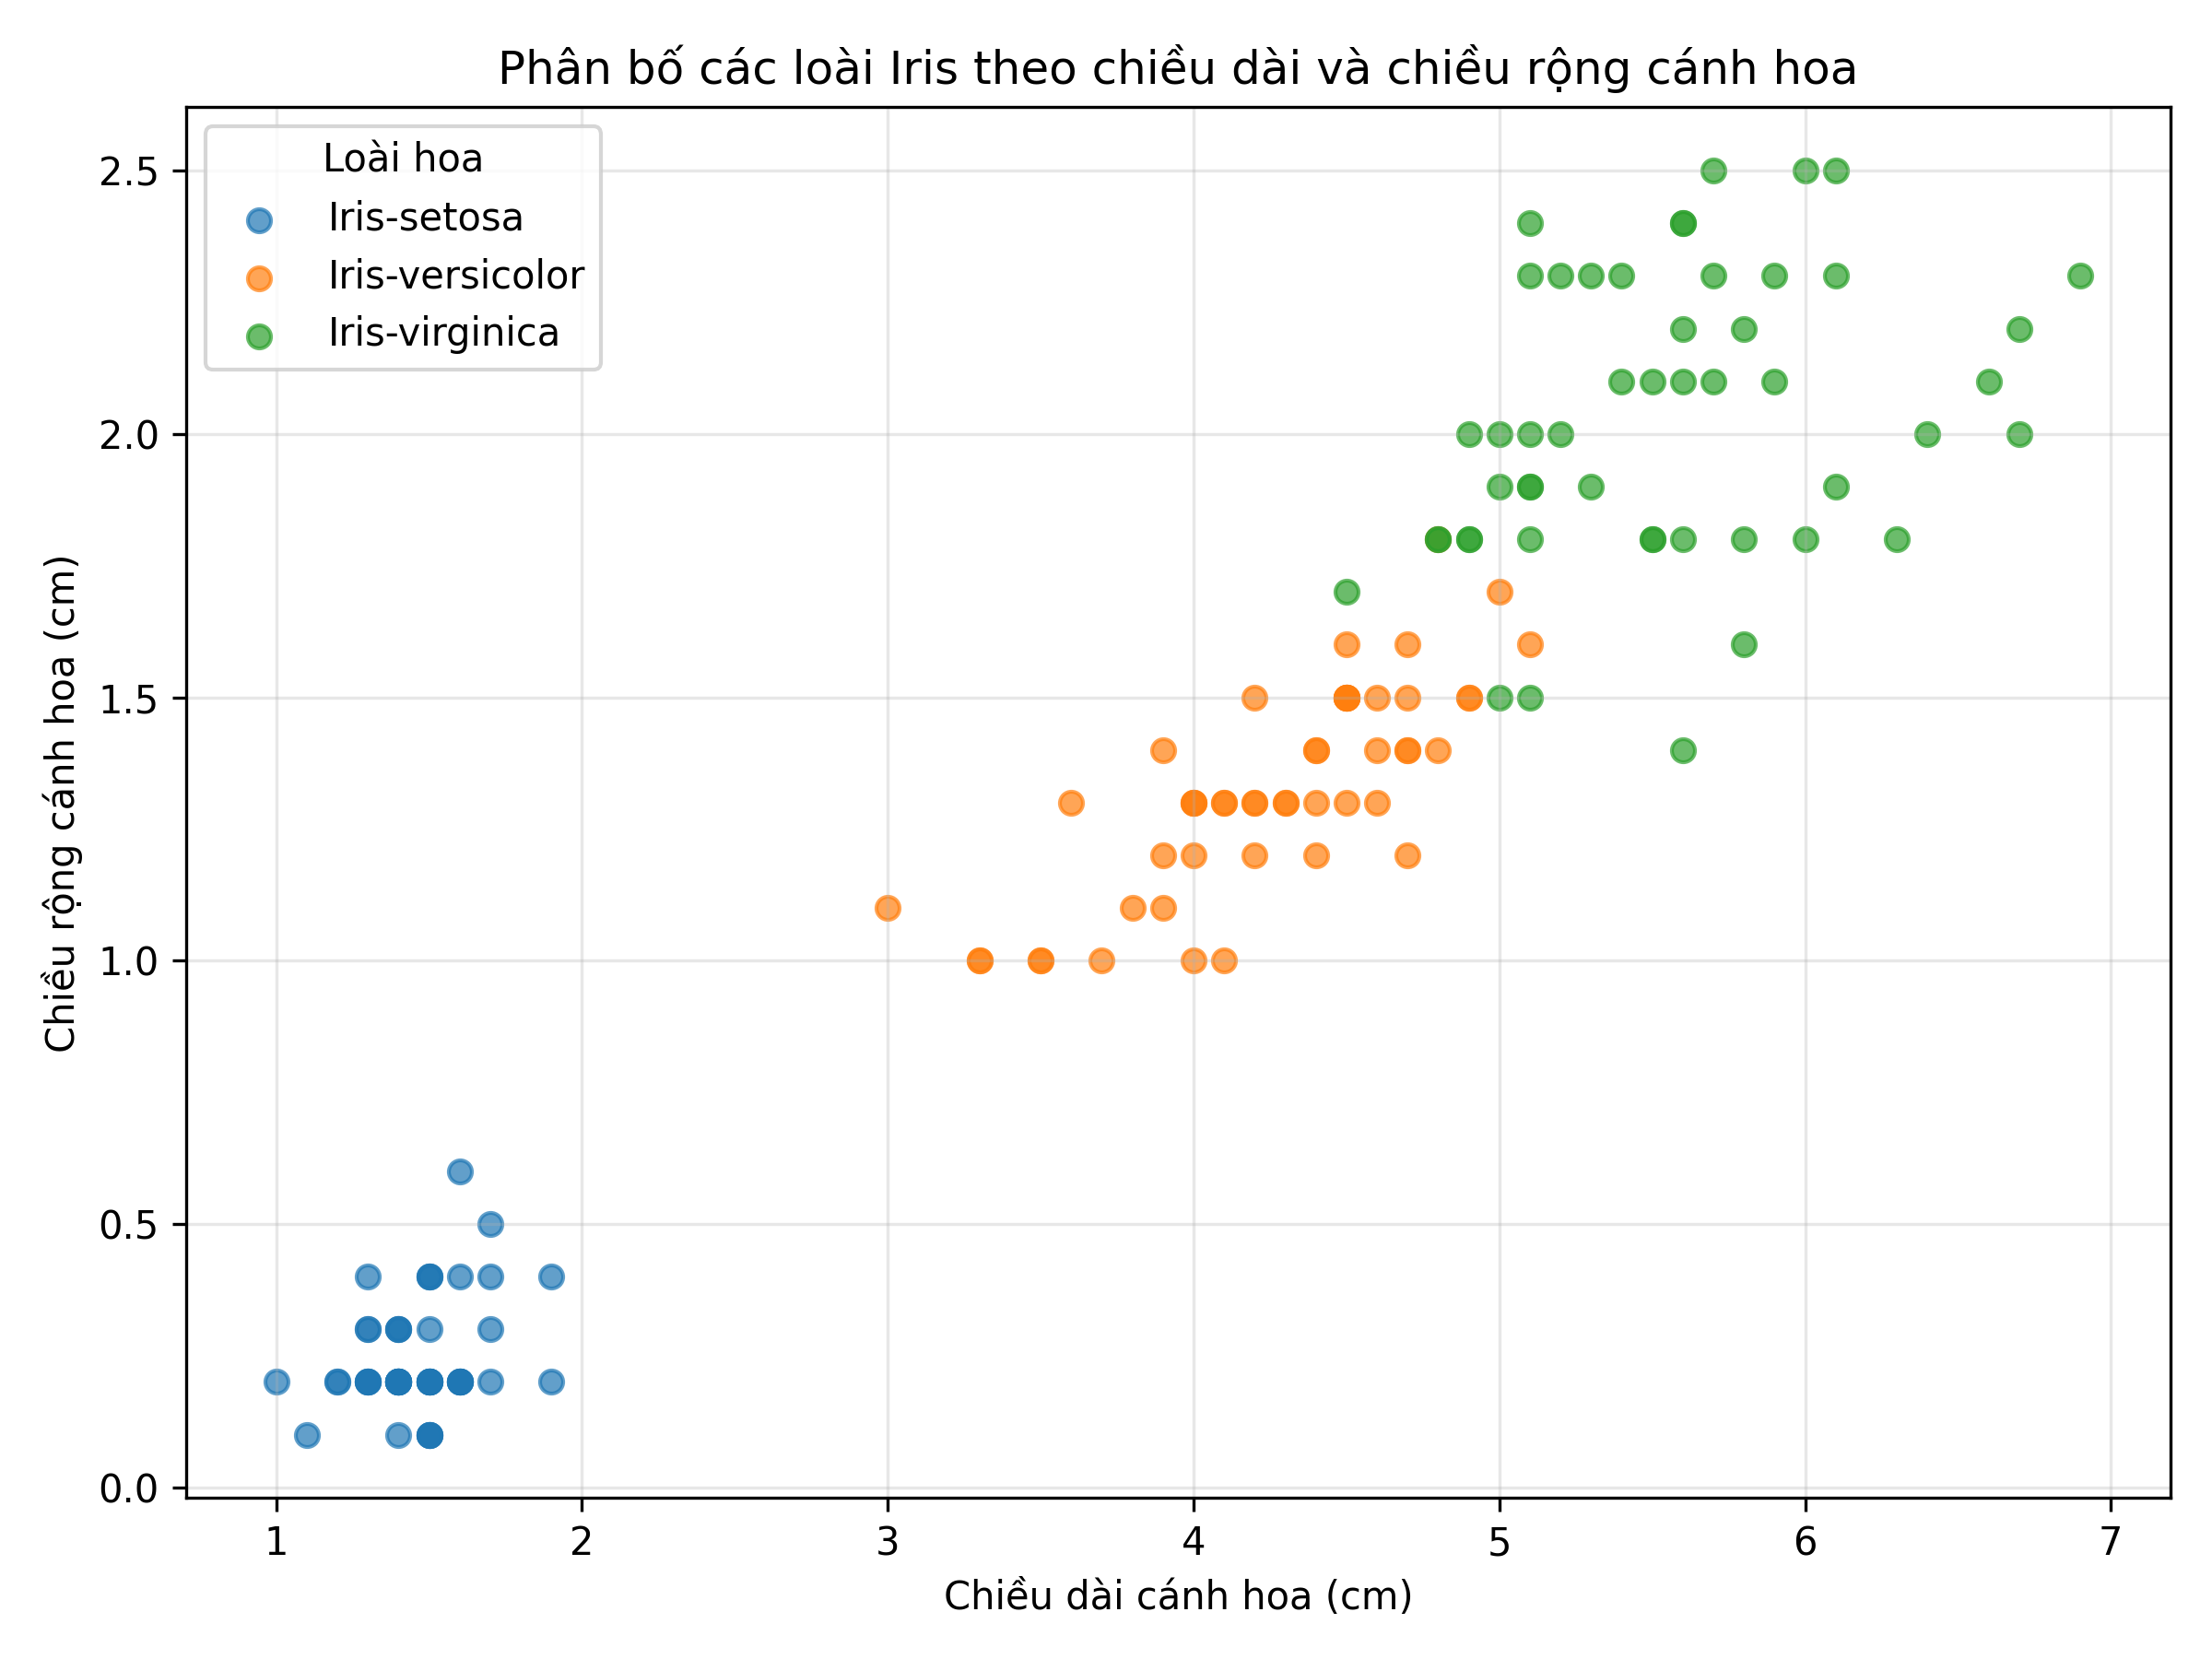
\includegraphics[width=0.85\textwidth]{iris_scatter.png}
		\caption{Biểu đồ phân tán giữa Petal Length và Petal Width theo ba loài hoa Iris}
		\label{fig:iris-scatter}
	\end{figure}
	
	\textit{Trục hoành: Petal Length (cm). Trục tung: Petal Width (cm). Mỗi màu đại diện cho một lớp Iris.}
	
	Khi quan sát biểu đồ, có thể phân tích ba nhóm dữ liệu dựa trên vị trí các điểm:
	
	\begin{itemize}
		\item \textbf{Iris Setosa:} Các điểm thường tập trung ở vùng có Petal Length và Petal Width nhỏ. Nhóm này có xu hướng tách biệt rõ hơn so với hai nhóm còn lại.
		
		\item \textbf{Iris Versicolor:} Các điểm tập trung ở vùng giá trị trung gian của hai đặc trưng cánh hoa.
		
		\item \textbf{Iris Virginica:} Các điểm thường xuất hiện ở vùng có Petal Length và Petal Width lớn hơn.
	\end{itemize}
	
	Biểu đồ cho thấy hai đặc trưng cánh hoa có khả năng hỗ trợ phân biệt ba loài hoa. Tuy nhiên, các điểm dữ liệu giữa Versicolor và Virginica có thể nằm gần nhau hoặc chồng lấn một phần. Điều này cho thấy việc phân loại hai lớp này đòi hỏi mô hình phải xem xét ranh giới phân chia một cách phù hợp.
	
	Cần phân biệt giữa biểu đồ trực quan hóa hai đặc trưng và không gian dữ liệu thực tế của mô hình. Biểu đồ chỉ biểu diễn Petal Length và Petal Width trên mặt phẳng hai chiều, trong khi mô hình SVM của dự án sử dụng cả bốn đặc trưng đầu vào. Do đó, hình minh họa không phải là toàn bộ ranh giới phân loại của mô hình SVM trong dự án.
	
	\subsection{Chuẩn bị dữ liệu cho quá trình huấn luyện}
	
	\subsubsection{Xác định ma trận đặc trưng và nhãn mục tiêu}
	
	Sau khi khảo sát dữ liệu, chương trình sử dụng hai thành phần \texttt{X} và \texttt{y} để đưa dữ liệu vào các thuật toán học máy:
	
	\begin{verbatim}
		X = iris.data
		y = iris.target
	\end{verbatim}
	
	Trong đó:
	
	\begin{itemize}
		\item \texttt{X}: Ma trận gồm 150 mẫu và 4 đặc trưng.
		\item \texttt{y}: Vector gồm 150 nhãn mục tiêu tương ứng.
	\end{itemize}
	
	Hai thành phần này được sử dụng chung trong quá trình huấn luyện SVM, LDA và KNN. Việc giữ nguyên cấu trúc dữ liệu giúp các mô hình được huấn luyện và kiểm tra trên cùng một tập mẫu, tạo cơ sở để so sánh kết quả đánh giá.
	
	\subsubsection{Chia tập huấn luyện và tập kiểm tra}
	
	Để đánh giá khả năng dự đoán của mô hình trên dữ liệu chưa được sử dụng trong quá trình huấn luyện, bộ dữ liệu được chia thành hai phần:
	
	\textbf{Tập huấn luyện (Training Set):} Là phần dữ liệu được sử dụng để thuật toán học mối quan hệ giữa các đặc trưng đầu vào và nhãn mục tiêu.
	
	\textbf{Tập kiểm tra (Testing Set):} Là phần dữ liệu được giữ riêng trong quá trình huấn luyện ban đầu, sau đó được sử dụng để kiểm tra khả năng dự đoán của mô hình trên các mẫu chưa tham gia vào bước học.
	
	Trong mã nguồn, thao tác chia dữ liệu được thực hiện bằng hàm \texttt{train\_test\_split()}:
	
	\begin{verbatim}
		from sklearn.model_selection import train_test_split
		
		X_train, X_test, y_train, y_test = train_test_split(
		X,
		y,
		test_size=0.2,
		random_state=42,
		stratify=y
		)
	\end{verbatim}
	
	Các tham số có ý nghĩa cụ thể:
	
	\textbf{Tham số \texttt{test\_size=0.2}}
	
	Tham số này quy định 20\% tổng số mẫu được dành cho tập kiểm tra, 80\% còn lại dành cho tập huấn luyện.
	
	Với 150 mẫu:
	
	\[
	N_{\text{test}}=150\times0,2=30
	\]
	
	\[
	N_{\text{train}}=150-30=120
	\]
	
	Do đó, tập huấn luyện có 120 mẫu và tập kiểm tra có 30 mẫu.
	
	\textbf{Tham số \texttt{random\_state=42}}
	
	Khi chia dữ liệu, hàm \texttt{train\_test\_split()} sử dụng cơ chế ngẫu nhiên để lựa chọn mẫu thuộc từng tập. Tham số \texttt{random\_state=42} cố định trạng thái sinh số ngẫu nhiên, giúp quá trình chia dữ liệu có thể được tái lập khi chạy lại chương trình với cùng dữ liệu và cấu hình.
	
	Giá trị 42 không phải là số lượng mẫu, tỷ lệ chia hay tham số của mô hình SVM. Đây chỉ là giá trị khởi tạo cho quá trình ngẫu nhiên.
	
	\textbf{Tham số \texttt{stratify=y}}
	
	Tham số này yêu cầu quá trình chia dữ liệu duy trì tỷ lệ các lớp theo vector nhãn ban đầu. Đây là điểm quan trọng đối với bài toán phân loại nhiều lớp, vì nếu chia ngẫu nhiên mà không xét đến nhãn, tỷ lệ giữa các lớp trong tập huấn luyện và tập kiểm tra có thể thay đổi.
	
	Vì mỗi lớp trong bộ Iris có 50 mẫu và tỷ lệ chia là 80:20, kết quả phân chia theo từng lớp là:
	
	\begin{itemize}
		\item Tập huấn luyện: 40 mẫu Setosa, 40 mẫu Versicolor và 40 mẫu Virginica.
		\item Tập kiểm tra: 10 mẫu Setosa, 10 mẫu Versicolor và 10 mẫu Virginica.
	\end{itemize}
	
	\begin{table}[htbp]
		\centering
		\caption{Kết quả phân chia dữ liệu theo từng lớp}
		\label{tab:iris-split}
		\begin{tabular}{|l|c|c|c|}
			\hline
			\textbf{Lớp hoa} &
			\textbf{Tập huấn luyện} &
			\textbf{Tập kiểm tra} &
			\textbf{Tổng số} \\
			\hline
			Iris Setosa & 40 & 10 & 50 \\
			\hline
			Iris Versicolor & 40 & 10 & 50 \\
			\hline
			Iris Virginica & 40 & 10 & 50 \\
			\hline
			\textbf{Tổng cộng} & \textbf{120} & \textbf{30} & \textbf{150} \\
			\hline
		\end{tabular}
	\end{table}
	
	Kết quả này cho thấy cả hai tập dữ liệu đều duy trì tỷ lệ ba lớp bằng nhau. Nhờ đó, việc đánh giá mô hình không bị lệch về số lượng mẫu giữa các lớp ngay từ bước phân chia dữ liệu.
	
	\subsubsection{Vai trò của tập huấn luyện và tập kiểm tra}
	
	Trong quá trình huấn luyện, mô hình sử dụng 120 mẫu thuộc tập huấn luyện để xác định quy luật phân loại.
	
	Sau khi hoàn thành bước học, mô hình nhận 30 mẫu thuộc tập kiểm tra để tạo ra các nhãn dự đoán. Các nhãn dự đoán được đối chiếu với nhãn thực tế tương ứng nhằm tính toán những chỉ số đánh giá.
	
	Ví dụ, nếu mô hình dự đoán đúng 30 trên tổng số 30 mẫu kiểm tra thì độ chính xác được tính:
	
	\[
	Accuracy=\frac{30}{30}\times100\%=100\%
	\]
	
	Nếu mô hình dự đoán đúng 29 trên 30 mẫu:
	
	\[
	Accuracy=\frac{29}{30}\times100\%\approx96,67\%
	\]
	
	Hai phép tính trên minh họa cách xác định Accuracy trên tập kiểm tra. Kết quả thực tế của từng mô hình sẽ được trình bày và phân tích ở Chương 4.
	
	Việc sử dụng tập kiểm tra riêng giúp hạn chế tình trạng chỉ đánh giá mô hình trên chính dữ liệu mà mô hình đã học. Tuy nhiên, kết quả từ một lần chia dữ liệu vẫn phụ thuộc vào cách chia mẫu cụ thể, do đó không thể xem một kết quả kiểm tra duy nhất là bằng chứng bảo đảm mô hình luôn đạt hiệu quả tương tự trên mọi bộ dữ liệu mới.
	
	\subsubsection{Phạm vi tiền xử lý dữ liệu trong dự án}
	
	Trong mã nguồn huấn luyện hiện tại, dữ liệu được tải trực tiếp từ \texttt{load\_iris()}, sau đó được tách thành ma trận đặc trưng \texttt{X} và vector nhãn \texttt{y}. Chương trình tiếp tục chia dữ liệu thành tập huấn luyện và tập kiểm tra trước khi đưa vào các mô hình.
	
	Quy trình hiện tại không thực hiện chuẩn hóa dữ liệu bằng \texttt{StandardScaler}, không loại bỏ ngoại lệ và không áp dụng phương pháp điền giá trị thiếu. Các giá trị đặc trưng được sử dụng trực tiếp từ bộ dữ liệu Iris của Scikit-learn.
	
	Việc không chuẩn hóa dữ liệu cần được lưu ý khi phân tích các thuật toán. SVM và KNN có thể chịu ảnh hưởng bởi sự khác biệt về thang đo giữa các đặc trưng. Đặc biệt, KNN sử dụng khoảng cách giữa các điểm dữ liệu để xác định những láng giềng gần nhất; vì vậy, đặc trưng có phạm vi giá trị lớn hơn có thể đóng góp nhiều hơn vào khoảng cách tính toán.
	
	Đối với SVM, thang đo đặc trưng cũng có thể ảnh hưởng đến cách xác định siêu phẳng và khoảng cách biên. Vì vậy, chuẩn hóa dữ liệu là một hướng cải tiến có thể xem xét trong các phiên bản tiếp theo. Tuy nhiên, báo cáo cần phân biệt rõ giữa quy trình đã triển khai và hướng cải tiến đề xuất; không được mô tả việc chuẩn hóa như một bước đã được thực hiện trong mã nguồn hiện tại.
	
	
	\section{XÂY DỰNG VÀ TRIỂN KHAI HỆ THỐNG IRIS BOTANICA AI}
	
	\subsection{Kiến trúc tổng thể của hệ thống}
	
	\noindent Sau khi hoàn thành quá trình khảo sát dữ liệu, huấn luyện và đánh giá các mô hình phân loại, đề tài tiến hành tích hợp các mô hình vào một ứng dụng Web với tên gọi \textbf{IRIS BOTANICA AI}. Hệ thống cho phép người dùng nhập bốn thông số hình thái của một mẫu hoa Iris, lựa chọn mô hình phân loại và nhận kết quả dự đoán trực tiếp thông qua giao diện Web.
	
	\noindent Hệ thống được xây dựng theo kiến trúc gồm các thành phần chính: giao diện Web (Frontend), Backend sử dụng FastAPI, các mô hình học máy SVM, LDA và KNN, cùng lớp xử lý dữ liệu và cơ sở dữ liệu. Trong đó, Frontend đảm nhận việc tiếp nhận thông tin và hiển thị kết quả; FastAPI xử lý yêu cầu từ người dùng, kiểm tra dữ liệu và điều phối việc gọi mô hình tương ứng. Các mô hình học máy thực hiện phân loại mẫu hoa dựa trên bốn đặc trưng đầu vào. Bên cạnh chức năng dự đoán, Backend còn xử lý các nghiệp vụ liên quan đến tài khoản người dùng, lịch sử dự đoán và kết quả đánh giá mô hình thông qua lớp truy cập cơ sở dữ liệu.
	
	\begin{figure}[tbph]
		\centering
		\includegraphics[width=0.95\textwidth]{"images/ảnh kiến trúc"}
		\caption{Kiến trúc tổng thể của hệ thống IRIS BOTANICA AI}
		\label{fig:anh-kien-truc}
	\end{figure}
	
	
	
	\noindent Luồng xử lý tổng quát của hệ thống được thực hiện theo trình tự:
	

	\begin{enumerate}[leftmargin=*]
		\item Người dùng truy cập giao diện Web IRIS BOTANICA AI.
		\item Người dùng đăng ký hoặc đăng nhập tài khoản nếu sử dụng các chức năng yêu cầu xác thực.
		\item Người dùng nhập bốn thông số hình thái của mẫu hoa Iris.
		\item Người dùng lựa chọn mô hình phân loại SVM, LDA hoặc KNN.
		\item Frontend gửi dữ liệu đến Backend thông qua API tương ứng.
		\item FastAPI kiểm tra cấu trúc dữ liệu đầu vào và chuyển dữ liệu thành mảng NumPy có kích thước $1\times4$.
		\item Backend gọi mô hình tương ứng đã được nạp từ tập tin lưu trữ để thực hiện dự đoán.
		\item Kết quả phân loại được chuyển về Frontend dưới dạng dữ liệu JSON.
		\item Backend thực hiện các thao tác ghi nhận kết quả dự đoán và thông tin liên quan vào cơ sở dữ liệu theo chức năng được gọi.
		\item Người dùng có thể xem kết quả dự đoán và truy cập các chức năng lịch sử hoặc đánh giá mô hình.
	\end{enumerate}
	
	\subsection{Chuẩn bị môi trường và cấu trúc dự án}
	\vspace{-0.3cm}
	\noindent Hệ thống được phát triển bằng ngôn ngữ Python. Môi trường lập trình được xây dựng nhằm phục vụ đồng thời ba nhóm nhiệm vụ: huấn luyện mô hình học máy, xây dựng Backend API và kết nối với cơ sở dữ liệu.
	
	\noindent Các công nghệ chính được sử dụng trong đề tài gồm:
	
	\begin{itemize}[leftmargin=*]
		\item \textbf{Python:} ngôn ngữ lập trình chính dùng để huấn luyện mô hình và xây dựng Backend.
		\item \textbf{Scikit-learn:} thư viện cung cấp thuật toán Support Vector Machine và các công cụ đánh giá mô hình.
		\item \textbf{Joblib:} thư viện dùng để lưu và nạp mô hình học máy.
		\item \textbf{FastAPI:} framework dùng để xây dựng các Web API.
		\item \textbf{Pydantic:} hỗ trợ kiểm tra và xác thực dữ liệu đầu vào cho API.
		\item \textbf{NumPy:} hỗ trợ chuyển đổi dữ liệu đầu vào thành cấu trúc mảng phù hợp với mô hình.
		\item \textbf{SQLAlchemy:} hỗ trợ kết nối và thực hiện các thao tác với cơ sở dữ liệu.
		\item \textbf{SQLite:} cơ sở dữ liệu được sử dụng để lưu trữ thông tin của hệ thống.
		\item \textbf{HTML, CSS và JavaScript:} xây dựng giao diện và xử lý tương tác phía người dùng.
		\item \textbf{Uvicorn:} máy chủ ASGI dùng để chạy ứng dụng FastAPI.
		\item \textbf{Render:} nền tảng triển khai ứng dụng trực tuyến.
	\end{itemize}
	
	\noindent Cấu trúc dự án được tổ chức thành các thành phần riêng biệt nhằm thuận tiện cho việc phát triển và bảo trì hệ thống. Các thành phần quan trọng gồm tập tin huấn luyện mô hình, tập tin mô hình đã lưu, mã nguồn FastAPI, các thành phần kết nối cơ sở dữ liệu và giao diện Web.
	\noindent Ngoài mô hình SVM, hệ thống còn tích hợp hai thuật toán phân loại khác là Linear Discriminant Analysis (LDA) và K-Nearest Neighbors (KNN) nhằm mở rộng khả năng lựa chọn mô hình khi thực hiện dự đoán trên giao diện Web. Ba mô hình được xây dựng và đánh giá bằng chương trình \texttt{evaluate\_models.py} trên cùng tập dữ liệu Iris và cùng cách chia tập huấn luyện, kiểm thử. Cụ thể, tập huấn luyện gồm 120 mẫu và tập kiểm thử gồm 30 mẫu. Sau khi hoàn thành đánh giá, mỗi mô hình được huấn luyện lại trên toàn bộ 150 mẫu và lưu thành tập tin riêng để phục vụ quá trình triển khai.
	
	\noindent Việc tích hợp LDA và KNN không thay đổi vai trò của SVM trong đề tài, mà cung cấp thêm cơ sở để so sánh kết quả phân loại giữa các thuật toán trên cùng bộ dữ liệu.
	
	
	\subsection{Huấn luyện và đánh giá mô hình SVM}
	
	\noindent Quá trình huấn luyện mô hình SVM đã được trình bày chi tiết ở Chương 2. Trong Chương 3, kết quả của quá trình này được sử dụng làm đầu vào cho giai đoạn triển khai hệ thống.
	
	\noindent Mô hình được xây dựng bằng lớp \texttt{SVC} của thư viện Scikit-learn với lựa chọn:
	
	\begin{lstlisting}[language=Python, numbers=none]
		model = SVC(kernel="linear")
	\end{lstlisting}
	
	\noindent Dữ liệu được chia thành tập huấn luyện và tập kiểm thử theo tỷ lệ 80/20, đồng thời sử dụng \texttt{stratify=y} để duy trì tỷ lệ các lớp. Kết quả kiểm thử của mô hình trên 30 mẫu thuộc tập Test đạt độ chính xác 100\% theo thực nghiệm của đề tài.
	
	\noindent Cần phân biệt rõ hai giai đoạn. Tập Test được sử dụng để đánh giá khả năng tổng quát hóa của mô hình, trong khi sau khi hoàn thành đánh giá, mô hình được huấn luyện lại trên toàn bộ 150 mẫu để tạo phiên bản cuối cùng phục vụ triển khai Web.
	
	\subsection{Xây dựng đường phân chia tuyến tính}
	
	\noindent Một trong những nội dung quan trọng của đề tài là trực quan hóa đường phân chia do mô hình SVM tạo ra. Với SVM sử dụng Kernel tuyến tính, ranh giới quyết định được biểu diễn dưới dạng một siêu phẳng:
	
	$$
	w^T x+b=0
	$$
	
	\noindent Trong đó, $x$ là vector đặc trưng của một mẫu dữ liệu, $w$ là vector trọng số và $b$ là hệ số dịch. Với dữ liệu hai chiều, phương trình trên tương ứng với một đường thẳng. Đối với dữ liệu Iris có bốn đặc trưng, ranh giới phân loại thực tế tồn tại trong không gian bốn chiều và có thể được gọi là siêu phẳng phân chia.\\
	
	\noindent Do không gian dữ liệu Iris có bốn chiều nên không thể biểu diễn trực tiếp toàn bộ siêu phẳng trên một mặt phẳng hai chiều. Vì vậy, đề tài sử dụng các cặp đặc trưng tiêu biểu để trực quan hóa xu hướng phân tách của các lớp dữ liệu.\\
	
	\noindent Đặc biệt, hai đặc trưng \text{petal length} và \text{petal width} thể hiện khả năng phân biệt rõ giữa các loài Iris. Việc trực quan hóa giúp minh họa trực quan nguyên lý hoạt động của SVM: tìm ranh giới có khả năng phân tách các nhóm dữ liệu với khoảng cách lề phù hợp.
	
	\begin{figure}[tbph]
		\centering
		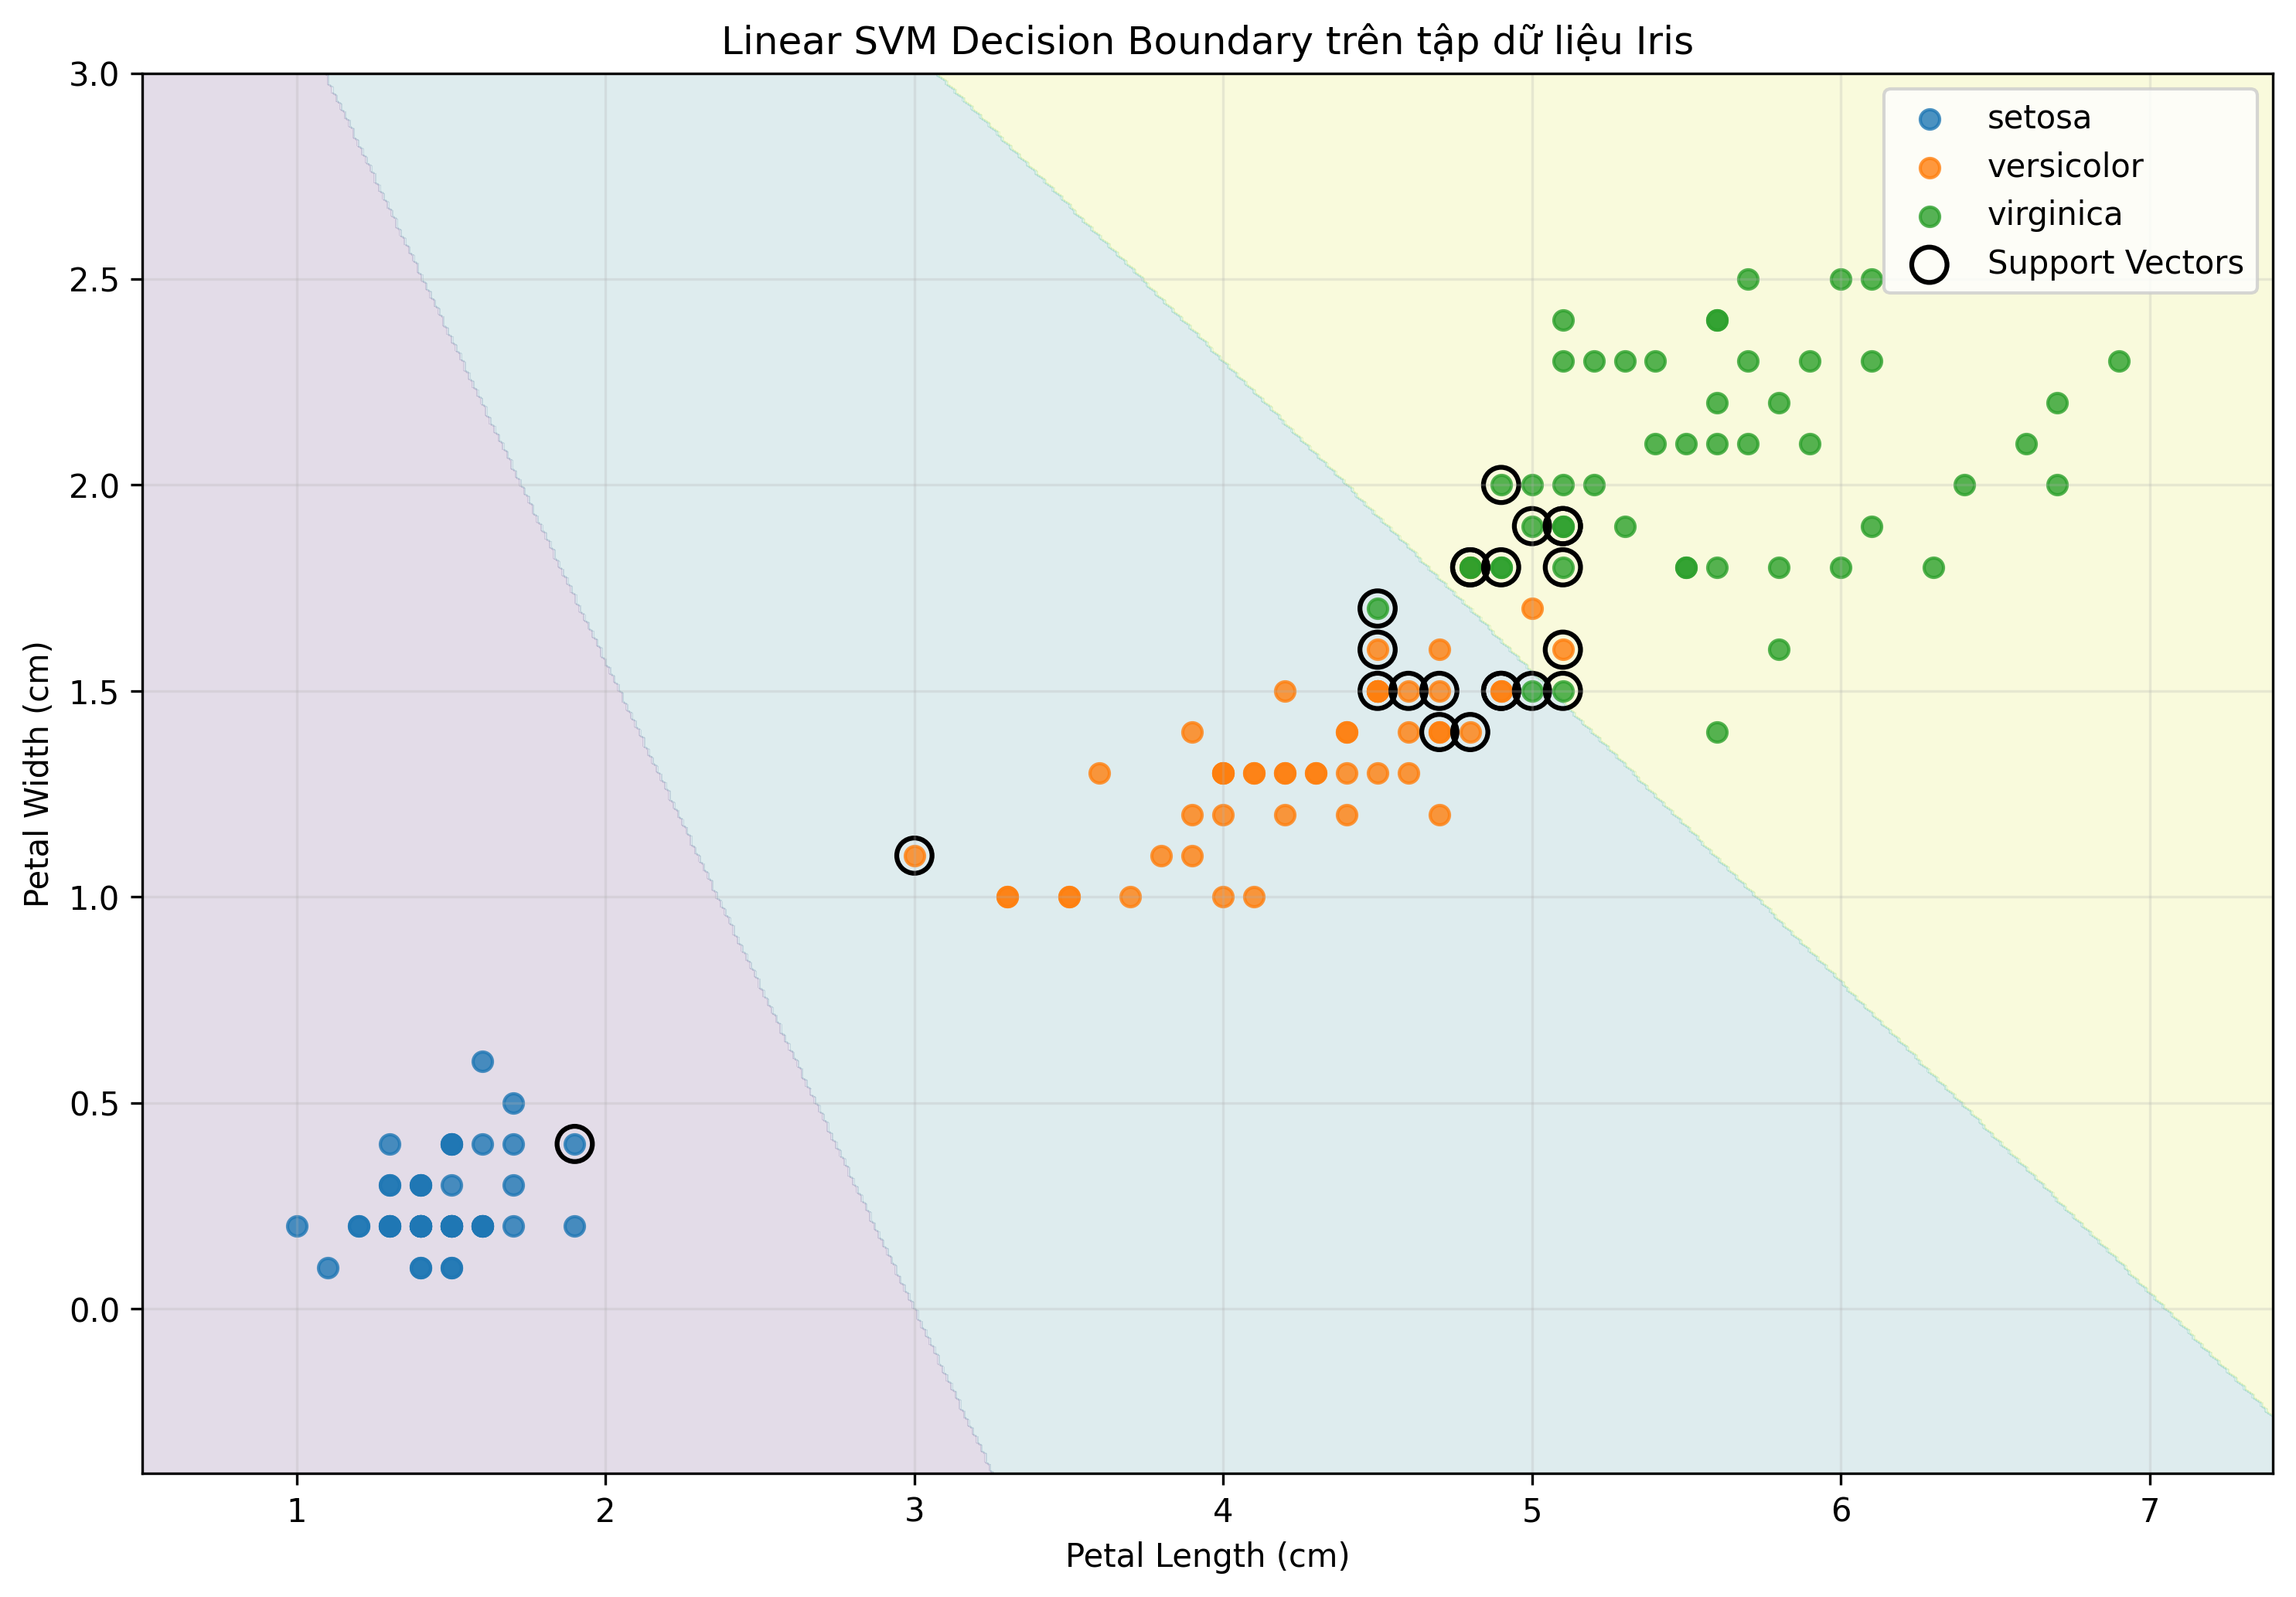
\includegraphics[width=0.7\textwidth]{images/linear_decision_boundary}
		\caption{Trực quan hóa đường phân chia tuyến tính trên dữ liệu Iris}
		\label{fig:lineardecisionboundary}
	\end{figure}
	
	
	\noindent Đường phân chia tuyến tính không phải là một bước huấn luyện riêng biệt sau khi mô hình đã được lưu. Đây là cách trực quan hóa và phân tích ranh giới quyết định được hình thành từ quá trình huấn luyện SVM. Do đó, quy trình hợp lý là: dữ liệu được sử dụng để huấn luyện mô hình, mô hình tạo ra các tham số phân loại, sau đó các tham số này được sử dụng để trực quan hóa đường phân chia và cuối cùng mô hình được lưu để triển khai.
	
	\subsection{Lưu và sử dụng mô hình}
	
	\noindent Sau khi đánh giá mô hình, phiên bản cuối cùng được huấn luyện trên toàn bộ tập dữ liệu Iris gồm 150 mẫu. Mô hình sau khi huấn luyện được lưu dưới dạng tập tin nhị phân \text{svm model.pkl} bằng thư viện Joblib.
	
	\begin{lstlisting}[language=Python, numbers=none]
		final_model = SVC(kernel="linear")
		final_model.fit(X, y)
		
		joblib.dump(final_model, "svm_model.pkl")
	\end{lstlisting}
	
\noindent Sau khi hoàn thành quá trình đánh giá, các mô hình được huấn luyện lại trên toàn bộ tập dữ liệu Iris gồm 150 mẫu. Mỗi mô hình được lưu thành một tập tin riêng bằng thư viện Joblib, cụ thể gồm \texttt{svm\_model.pkl}, \texttt{lda\_model.pkl} và \texttt{knn\_model.pkl}.

\begin{lstlisting}[language=Python, numbers=none]
	joblib.dump(svm_model, "svm_model.pkl")
	joblib.dump(lda_model, "lda_model.pkl")
	joblib.dump(knn_model, "knn_model.pkl")
\end{lstlisting}

\noindent Khi Backend khởi động, các tập tin mô hình được nạp vào bộ nhớ để sẵn sàng phục vụ yêu cầu dự đoán. Việc nạp mô hình trước giúp hệ thống không phải thực hiện lại quá trình huấn luyện mỗi khi người dùng gửi yêu cầu.

\begin{lstlisting}[language=Python, numbers=none]
	models = {
		"SVM": joblib.load("svm_model.pkl"),
		"LDA": joblib.load("lda_model.pkl"),
		"KNN": joblib.load("knn_model.pkl")
	}
\end{lstlisting}

\noindent Nhờ cách tổ chức này, Backend có thể lựa chọn mô hình phù hợp dựa trên yêu cầu được gửi từ giao diện Web.
	
	
	\noindent
	Sau khi khởi động hệ thống FastAPI, mô hình SVM được nạp tự động từ tệp
	\text{svm\_model.pkl} thông qua thư viện \texttt{joblib}. 
	Quá trình này được thực hiện thành công trước khi hệ thống tiếp nhận các yêu cầu dự đoán từ người dùng.
	\begin{lstlisting}[language=Python, caption={Nạp mô hình SVM khi khởi động hệ thống}]
		model = joblib.load("svm_model.pkl")
		print("Model svm_model.pkl loaded successfully!")
	\end{lstlisting}
	
	\subsection{Xây dựng API mô hình bằng FastAPI}
	
	\noindent Sau khi có mô hình đã lưu, FastAPI được sử dụng để xây dựng lớp API trung gian giữa giao diện Web và mô hình SVM. API có nhiệm vụ tiếp nhận dữ liệu, kiểm tra dữ liệu, gọi mô hình dự đoán và trả kết quả dưới dạng JSON.
	
	\subsubsection{Khởi tạo ứng dụng FastAPI}
	
	\noindent Ứng dụng được khởi tạo bằng lớp \text{FastAPI}. Mô hình SVM được nạp khi Backend khởi động để sẵn sàng phục vụ các yêu cầu dự đoán.
	
	\begin{lstlisting}[language=Python, numbers=none]
		app = FastAPI(
		title="Iris Flower Classification API",
		description="API for Iris flower classification using SVM model",
		version="1.0.0"
		)
		
		model = joblib.load("svm_model.pkl")
	\end{lstlisting}
	
	\subsubsection{Xây dựng API dự đoán}
	
\noindent Bên cạnh endpoint \texttt{/predict} sử dụng mô hình SVM, hệ thống còn cung cấp endpoint \texttt{/predict-model} nhằm hỗ trợ lựa chọn mô hình phân loại. Endpoint này tiếp nhận bốn thông số hình thái của mẫu hoa cùng thông tin xác định mô hình được lựa chọn. Backend căn cứ vào tên mô hình để gọi bộ phân loại tương ứng trong nhóm mô hình đã được nạp trước đó.

\noindent Cách tổ chức này cho phép người dùng thực hiện dự đoán bằng ba thuật toán SVM, LDA và KNN thông qua cùng một hệ thống Backend, thay vì phải xây dựng một ứng dụng riêng cho từng mô hình. Kết quả trả về được sử dụng để hiển thị loài hoa dự đoán trên giao diện Web.
	\newpage
	\begin{lstlisting}[language=Python, numbers=none]
		@app.post("/predict")
		def predict_iris(data: IrisInput):
		
		
		input_features = np.array([[
		data.sepal_length,
		data.sepal_width,
		data.petal_length,
		data.petal_width
		]])
		
		prediction_id = int(model.predict(input_features)[0])
		predicted_class = CLASS_NAMES[prediction_id]
		
		return {
			"input": {
				"sepal_length": data.sepal_length,
				"sepal_width": data.sepal_width,
				"petal_length": data.petal_length,
				"petal_width": data.petal_width
			},
			"prediction_id": prediction_id,
			"predicted_class": predicted_class
		}
		
		
	\end{lstlisting}
	
	\noindent Dữ liệu đầu vào được chuyển thành mảng NumPy có kích thước $1\times4$, phù hợp với cấu trúc dữ liệu mà mô hình Scikit-learn yêu cầu.
	
	\subsubsection{Kiểm tra dữ liệu đầu vào}
	
	\noindent Pydantic được sử dụng để định nghĩa cấu trúc dữ liệu đầu vào. Các trường dữ liệu được khai báo dưới dạng số thực và yêu cầu giá trị lớn hơn 0.
	
	\begin{lstlisting}[language=Python, numbers=none]
		class IrisInput(BaseModel):
		sepal_length: float = Field(..., gt=0)
		sepal_width: float = Field(..., gt=0)
		petal_length: float = Field(..., gt=0)
		petal_width: float = Field(..., gt=0)
	\end{lstlisting}
	
	\noindent Cơ chế này giúp hạn chế dữ liệu không hợp lệ trước khi dữ liệu được chuyển tới mô hình học máy.
	
	\begin{figure}[tbph]
		\centering
		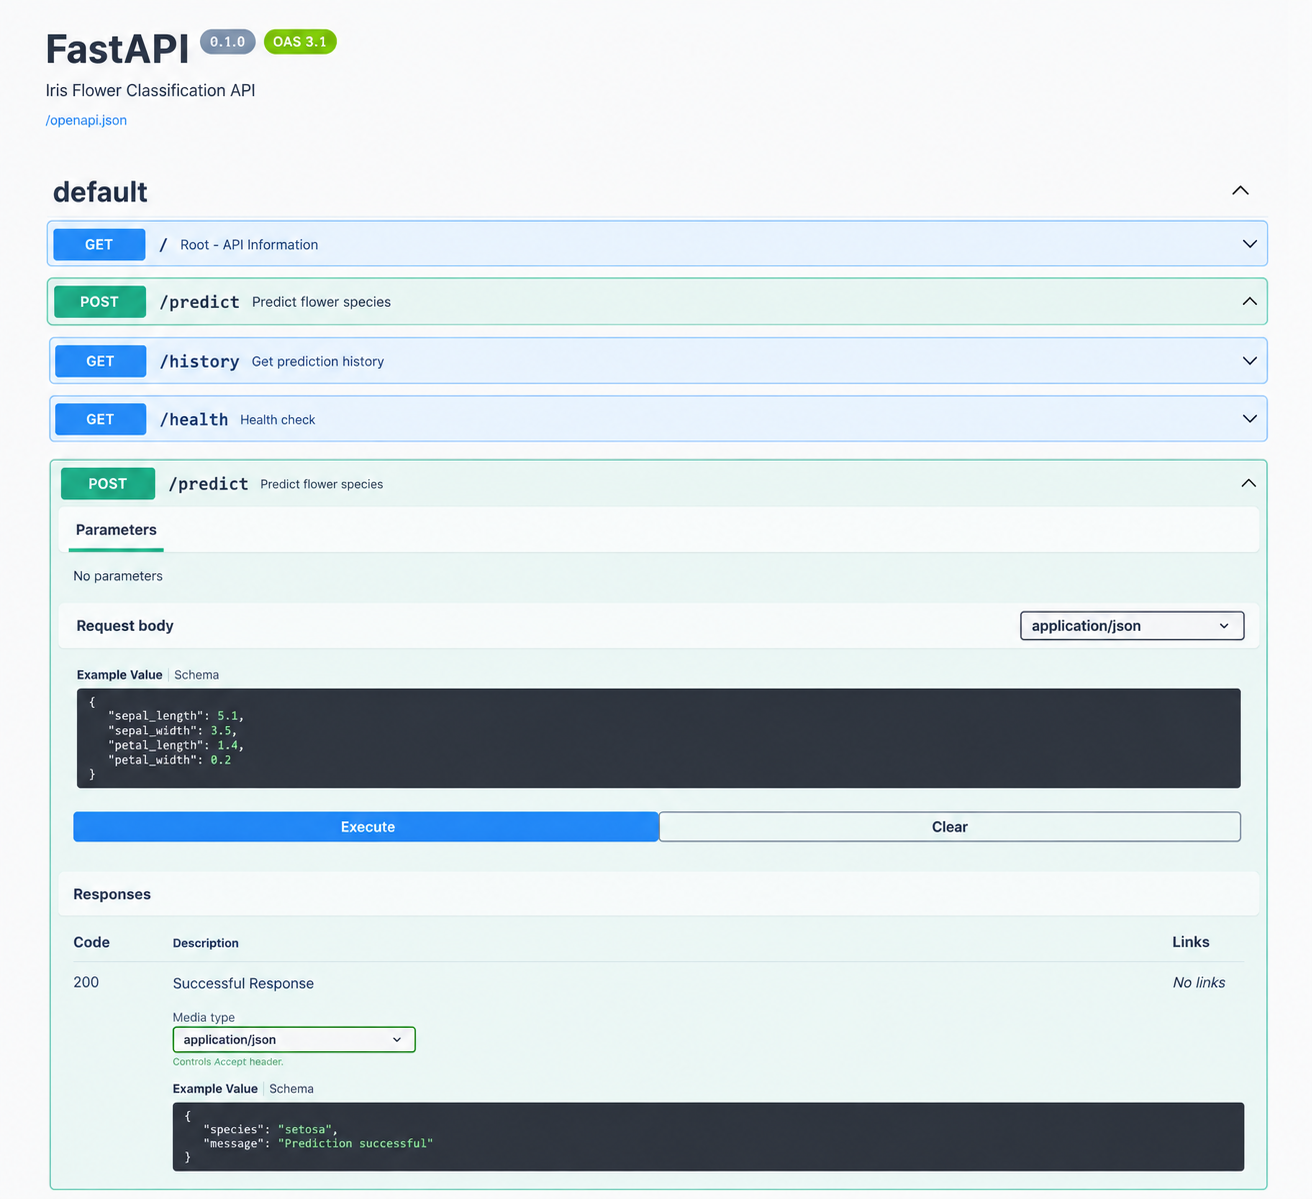
\includegraphics[width=0.5\textwidth]{images/api_predict.png}
		\caption{API dự đoán hoa Iris trên Swagger UI}
		\label{fig:apipredict}
	\end{figure}
	
	
	\subsection{Xây dựng API CSDL}
	
	\noindent Bên cạnh API phục vụ dự đoán, hệ thống còn xây dựng lớp API phục vụ trao đổi dữ liệu với cơ sở dữ liệu. Việc tách riêng chức năng này giúp Backend quản lý rõ ràng hai nhóm nhiệm vụ: xử lý mô hình học máy và xử lý dữ liệu hệ thống.
	
	\noindent API CSDL được sử dụng để thực hiện các thao tác như tạo tài khoản, kiểm tra thông tin đăng nhập, lưu lịch sử dự đoán và truy vấn lịch sử của người dùng.
	
	\noindent Quy trình trao đổi dữ liệu có thể khái quát:
	
	$$
	\text{Web} \rightarrow \text{API} \rightarrow \text{Database Layer} \rightarrow \text{SQLite}
	$$
	
	\noindent Khi người dùng thực hiện một thao tác yêu cầu lưu hoặc truy xuất dữ liệu, Frontend gửi yêu cầu đến Backend. Backend tiếp nhận yêu cầu, thực hiện kiểm tra và sử dụng lớp kết nối CSDL để thực hiện câu lệnh tương ứng.
	
	\begin{figure}[htbp]
		\centering
		
		\begin{tikzpicture}[
			node distance=1.8cm,
			box/.style={
				draw,
				rounded corners=2pt,
				minimum width=5.5cm,
				minimum height=0.9cm,
				align=center,
				font=\small
			}
			]
			
			\node[box] (web) {Web Iris Botanica AI};
			
			\node[box, below=1.8cm of web] (api)
			{FastAPI Backend\\API xử lý dữ liệu};
			
			\node[box, below=1.8cm of api] (dbapi)
			{Database API\\Kết nối và truy vấn};
			
			\node[box, below=1.8cm of dbapi] (database)
			{SQLite Database\\Người dùng -- Lịch sử -- Dự đoán};
			
			\draw[->, thick] (web) -- (api);
			\draw[->, thick] (api) -- (dbapi);
			\draw[->, thick] (dbapi) -- (database);
			
		\end{tikzpicture}
		
		\caption{Kiến trúc kết nối giữa Web, API và cơ sở dữ liệu}
		
	\end{figure}
	
	
	\subsection{Xây dựng hệ thống người dùng}
	
	\noindent Để hệ thống có khả năng phân biệt dữ liệu của từng người sử dụng, đề tài bổ sung cơ chế quản lý tài khoản. Người dùng có thể tạo tài khoản, đăng nhập và sử dụng các chức năng dự đoán trên hệ thống.
	
	\subsubsection{Đăng ký tài khoản}
	
	\noindent Khi người dùng đăng ký, hệ thống tiếp nhận tên đăng nhập và mật khẩu. Backend kiểm tra thông tin trước khi lưu vào cơ sở dữ liệu. Nếu tên đăng nhập đã tồn tại, hệ thống trả về thông báo tương ứng thay vì tạo bản ghi trùng lặp.
	
	\noindent Việc lưu tài khoản vào CSDL giúp thông tin người dùng được duy trì giữa các lần sử dụng ứng dụng.
	
	\begin{figure}[tbph]
		\centering
		\includegraphics[width=0.65\textwidth]{"images/đăng ký"}
		\caption{Giao diện đăng ký tài khoản, yêu cầu 8 chữ số}
		\label{fig:ang-ky}
	\end{figure}
	
	
	
	\subsubsection{Đăng nhập}
	
	\noindent Sau khi có tài khoản, người dùng có thể đăng nhập bằng tên đăng nhập và mật khẩu. Backend kiểm tra thông tin với dữ liệu được lưu trong cơ sở dữ liệu. Nếu thông tin chính xác, hệ thống tạo trạng thái đăng nhập cho người dùng.
	
	\begin{figure}[tbph]
		\centering
		\includegraphics[width=0.65\textwidth]{"images/đăng nhập"}
		\caption{Giao diện đăng nhập hệ thống}
		\label{fig:ang-nhap}
	\end{figure}
	
	
	\subsubsection{Quản lý phiên đăng nhập}
	
	\noindent Sau khi đăng nhập thành công, hệ thống cần duy trì trạng thái người dùng trong phiên làm việc. Cơ chế phiên giúp Backend xác định người dùng hiện tại khi người dùng thực hiện các thao tác tiếp theo như dự đoán hoặc xem lịch sử.
	
	\noindent Việc quản lý phiên cũng giúp hệ thống gắn kết dữ liệu lịch sử dự đoán với đúng tài khoản đang sử dụng, thay vì lưu dữ liệu một cách không phân biệt.
	
	\subsection{Xây dựng chức năng lưu trữ lịch sử dự đoán}
	
	\noindent Một trong những chức năng mở rộng của hệ thống là lưu lại các lần dự đoán. Mỗi khi người dùng thực hiện dự đoán, hệ thống có thể ghi nhận thông tin đầu vào, kết quả dự đoán, tài khoản thực hiện và thời gian xử lý.
	
	\subsubsection{Lưu kết quả dự đoán}
	
	\noindent Sau khi mô hình SVM trả về kết quả, Backend thực hiện quá trình lưu dữ liệu vào cơ sở dữ liệu. Việc lưu trữ được thực hiện sau khi quá trình dự đoán hoàn thành để đảm bảo dữ liệu lịch sử phản ánh đúng kết quả mà hệ thống đã trả về.
	
	\noindent Thông tin lịch sử có thể bao gồm:
	
	\begin{itemize}[leftmargin=*]
		\item Tài khoản thực hiện dự đoán.
		\item Bốn thông số đầu vào của mẫu hoa.
		\item Loài hoa được dự đoán.
		\item Mã mô hình được sử dụng.
		\item Thời gian thực hiện dự đoán.
		\item Thời gian chạy mô hình.
		\item Trạng thái bản ghi.
	\end{itemize}
	
	\subsubsection{Xem lịch sử dự đoán}
	
	\noindent Người dùng sau khi đăng nhập có thể truy cập chức năng lịch sử để xem lại các lần dự đoán trước đó. Dữ liệu được truy vấn dựa trên tài khoản đang đăng nhập, giúp mỗi người dùng chỉ xem được dữ liệu thuộc phạm vi được hệ thống cho phép.
	
	\begin{figure}[tbph]
		\centering
		\includegraphics[width=0.90\textwidth]{"images/lịch sử dự đoán"}
		\caption{Giao diện hiển thị lịch sử dự đoán}
		\label{fig:lich-su-du-oan}
	\end{figure}
	
	
	\subsubsection{Xóa mềm và khôi phục dữ liệu}
	
	\noindent Đối với những bản ghi lịch sử không còn cần hiển thị, hệ thống có thể sử dụng cơ chế xóa mềm. Thay vì xóa ngay dữ liệu khỏi cơ sở dữ liệu, bản ghi được chuyển sang trạng thái không hoạt động.
	
	\noindent Cách tiếp cận này giúp hạn chế mất dữ liệu ngoài ý muốn và tạo khả năng khôi phục bản ghi khi cần thiết.
	
	\subsubsection{Xóa vĩnh viễn}
	
	\noindent Trong trường hợp người dùng hoặc hệ thống xác định một bản ghi không còn cần thiết, dữ liệu có thể được xóa vĩnh viễn khỏi cơ sở dữ liệu. Chức năng này được tách biệt với xóa mềm nhằm tránh việc xóa dữ liệu ngoài ý muốn trong thao tác thông thường.
	
	\subsection{Ghi nhận thời gian chạy mô hình}
	
	\noindent Ngoài kết quả dự đoán, hệ thống còn ghi nhận thời gian thực hiện mô hình nhằm phục vụ đánh giá hiệu năng của quá trình suy luận.
	
	\noindent Quy trình đo thời gian được thực hiện theo nguyên tắc:
	
	$$
	T_{\text{chạy}} =
	T_{\text{kết thúc}} -
	T_{\text{bắt đầu}}
	$$
	
	\noindent Trong đó thời điểm bắt đầu được ghi nhận trước khi gọi hàm dự đoán và thời điểm kết thúc được ghi nhận sau khi mô hình trả về kết quả.
	
	\begin{lstlisting}[language=Python, numbers=none]
		import time
		
		start_time = time.perf_counter()
		
		prediction_id = int(model.predict(input_features)[0])
		
		end_time = time.perf_counter()
		
		runtime = end_time - start_time
	\end{lstlisting}
	
	\noindent Thông tin thời gian chạy có thể được lưu cùng kết quả dự đoán để phục vụ quá trình theo dõi hiệu năng hệ thống.
	
	\noindent Trong báo cáo, thời gian chạy cần được trình bày dựa trên kết quả đo thực tế của hệ thống thay vì sử dụng một giá trị cố định không có nguồn đo.
	
	\subsection{Kết nối hệ thống với cơ sở dữ liệu}
	
	\noindent Cơ sở dữ liệu đóng vai trò lưu trữ dữ liệu phát sinh trong quá trình vận hành hệ thống. Trong phạm vi đề tài, SQLite được sử dụng do có cấu trúc đơn giản, không yêu cầu triển khai một máy chủ CSDL riêng và phù hợp với quy mô dữ liệu của ứng dụng.
	
	\noindent Lớp kết nối được tổ chức riêng nhằm giúp các module khác của hệ thống có thể sử dụng lại kết nối CSDL mà không phải viết lại toàn bộ logic kết nối.
	
	\noindent Kiến trúc xử lý dữ liệu có thể mô tả:
	
	\begin{figure}[htbp]
		\centering
		\begin{tikzpicture}[
			node distance=1.3cm,
			box/.style={
				draw,
				rounded corners,
				minimum width=3cm,
				minimum height=1cm,
				align=center
			}
			]
			
			\node (web) [box] {Web\\Frontend};
			
			\node (api) [box, right=of web, xshift=1cm]
			{FastAPI\\Backend};
			
			\node (dbapi) [box, right=of api, xshift=1cm]
			{Database\\Layer};
			
			\node (db) [box, right=of dbapi, xshift=1cm]
			{SQLite\\Database};
			
			\draw[->, thick] (web) -- (api);
			\draw[->, thick] (api) -- (dbapi);
			\draw[->, thick] (dbapi) -- (db);
			
		\end{tikzpicture}
		\caption{Luồng kết nối giữa Web, Backend và cơ sở dữ liệu}
		\label{fig:database-flow}
	\end{figure}
	
	
	
	\noindent Sự phân tách này giúp hệ thống có cấu trúc rõ ràng hơn và thuận tiện khi mở rộng sang hệ quản trị cơ sở dữ liệu khác trong tương lai.
	
	\subsection{Xây dựng giao diện Web IRIS BOTANICA AI}
	
	\noindent Giao diện Web là lớp tương tác trực tiếp với người dùng. Thiết kế của hệ thống hướng đến việc đơn giản hóa thao tác: người dùng không cần biết cách mô hình SVM hoạt động bên trong mà chỉ cần cung cấp các thông số của mẫu hoa.
	
	\noindent Giao diện chính cung cấp các khu vực nhập bốn thông số:
	
	\begin{itemize}[leftmargin=*]
		\item Chiều dài đài hoa.
		\item Chiều rộng đài hoa.
		\item Chiều dài cánh hoa.
		\item Chiều rộng cánh hoa.
	\end{itemize}
	
	\noindent Sau khi người dùng thực hiện dự đoán, giao diện nhận phản hồi từ API và hiển thị tên loài hoa tương ứng.
	
	\begin{figure}[tbph]
		\centering
		\includegraphics[width=0.92\textwidth]{"images/web chính"}
		\caption{Giao diện chính của hệ thống IRIS BOTANICA AI}
		\label{fig:web-chinh}
	\end{figure}
	
	\noindent Giao diện Web được xây dựng bằng HTML, CSS và JavaScript. JavaScript đảm nhận việc lấy dữ liệu từ biểu mẫu, gửi yêu cầu đến Backend bằng HTTP và nhận dữ liệu JSON để cập nhật nội dung trên giao diện mà không cần tải lại toàn bộ trang.
	
	\subsection{Quy trình triển khai từ mô hình đến Web}
	
	\noindent Một trong những mục tiêu quan trọng của đề tài là không chỉ xây dựng một mô hình học máy độc lập mà còn đưa mô hình vào một sản phẩm có khả năng sử dụng thực tế. Vì vậy, quá trình triển khai được thực hiện theo một chuỗi các bước liên kết.
	
	\begin{figure}[htbp]
		\centering
		\begin{tikzpicture}[
			node distance=0.65cm,
			every node/.style={
				draw,
				rounded corners,
				align=center,
				minimum width=4.4cm,
				minimum height=0.7cm,
				font=\small
			},
			arrow/.style={->, thick}
			]
			
			
			\node (data) {1. Chuẩn bị dữ liệu Iris};
			\node (train) [below=of data] {2. Huấn luyện mô hình SVM};
			\node (eval) [below=of train] {3. Đánh giá mô hình};
			\node (boundary) [below=of eval] {4. Trực quan hóa đường phân chia};
			\node (save) [below=of boundary] {5. Lưu mô hình svm\_model.pkl};
			\node (api) [below=of save] {6. Xây dựng FastAPI};
			\node (db) [below=of api] {7. Xây dựng API và kết nối CSDL};
			\node (user) [below=of db] {8. Xây dựng hệ thống người dùng};
			\node (history) [below=of user] {9. Lưu lịch sử và thời gian chạy};
			\node (web) [below=of history] {10. Kết nối giao diện Web};
			\node (test) [below=of web] {11. Kiểm thử hệ thống};
			\node (deploy) [below=of test] {12. Triển khai trực tuyến};
			
			\draw[arrow] (data) -- (train);
			\draw[arrow] (train) -- (eval);
			\draw[arrow] (eval) -- (boundary);
			\draw[arrow] (boundary) -- (save);
			\draw[arrow] (save) -- (api);
			\draw[arrow] (api) -- (db);
			\draw[arrow] (db) -- (user);
			\draw[arrow] (user) -- (history);
			\draw[arrow] (history) -- (web);
			\draw[arrow] (web) -- (test);
			\draw[arrow] (test) -- (deploy);
			
		\end{tikzpicture}
		\caption{Quy trình triển khai từ mô hình học máy đến ứng dụng Web}
		
		```
		
	\end{figure}
	\newpage
	\noindent Quy trình trên thể hiện mối liên hệ giữa phần học máy và phần phát triển phần mềm. Trong đó, mô hình SVM là thành phần trung tâm của chức năng dự đoán, còn FastAPI đóng vai trò cầu nối giữa mô hình, cơ sở dữ liệu và giao diện Web.
	
	\subsubsection*{Bước 1 -- Chuẩn bị dữ liệu}
	
	\noindent Tập dữ liệu Iris được nạp bằng Scikit-learn và gồm 150 mẫu thuộc ba lớp. Bốn đặc trưng được sử dụng làm đầu vào cho mô hình.
	
	\subsubsection*{Bước 2 -- Huấn luyện SVM}
	
	\noindent Mô hình \texttt{SVC(kernel="linear")} được huấn luyện trên tập Train. Sau đó mô hình được đánh giá bằng tập Test độc lập.
	
	\subsubsection*{Bước 3 -- Đánh giá mô hình}
	
	\noindent Accuracy và các chỉ số đánh giá khác được sử dụng để kiểm tra khả năng phân loại. Confusion Matrix được sử dụng để quan sát trực quan số lượng mẫu được phân loại đúng hoặc nhầm giữa các lớp.
	
	\subsubsection*{Bước 4 -- Trực quan hóa đường phân chia}
	
	\noindent Sau khi mô hình được huấn luyện, các ranh giới quyết định được trực quan hóa nhằm minh họa cách SVM phân tách các nhóm dữ liệu.
	
	\subsubsection*{Bước 5 -- Lưu mô hình}
	
	\noindent Phiên bản mô hình cuối cùng được huấn luyện trên toàn bộ dữ liệu và lưu thành \texttt{svm model.pkl}.
	
	\subsubsection*{Bước 6 -- Xây dựng API mô hình}
	
	\noindent FastAPI được sử dụng để tạo endpoint \texttt{/predict}. Endpoint tiếp nhận dữ liệu từ Web, gọi mô hình và trả kết quả dưới dạng JSON.
	
	\subsubsection*{Bước 7 -- Kết nối CSDL}
	
	\noindent Hệ thống được bổ sung lớp xử lý dữ liệu và API CSDL nhằm lưu trữ thông tin người dùng, lịch sử dự đoán và các thông tin liên quan.
	
	\subsubsection*{Bước 8 -- Xây dựng hệ thống người dùng}
	
	\noindent Chức năng đăng ký, đăng nhập và quản lý phiên giúp hệ thống xác định người dùng đang thực hiện các thao tác.
	
	\subsubsection*{Bước 9 -- Lưu lịch sử và thời gian chạy}
	
	\noindent Sau mỗi lần dự đoán, kết quả và thời gian xử lý được ghi nhận vào hệ thống lưu trữ.
	
	\subsubsection*{Bước 10 -- Kết nối giao diện Web}
	
	\noindent Frontend gửi dữ liệu đến API và nhận kết quả JSON để hiển thị trực quan cho người dùng.
	
	\subsubsection{Bước 11 -- Kiểm thử}
	
	\noindent Hệ thống được kiểm thử trước trên môi trường cục bộ bằng Uvicorn. Các chức năng chính được kiểm tra gồm đăng nhập, dự đoán, lưu lịch sử, truy vấn dữ liệu và xử lý dữ liệu không hợp lệ.
	
	\subsubsection*{Bước 12 -- Triển khai trực tuyến}
	
	\noindent Sau khi hoàn thành kiểm thử, ứng dụng được triển khai lên nền tảng Render để cung cấp khả năng truy cập thông qua Internet.
	
	\subsection{Kiểm thử và xử lý lỗi}
	
	\noindent Trong quá trình xây dựng hệ thống, việc kiểm thử được thực hiện theo từng lớp thay vì chỉ kiểm tra kết quả cuối cùng. Cách tiếp cận này giúp xác định chính xác vị trí phát sinh lỗi.
	
	\subsubsection{Kiểm thử Backend cục bộ}
	
	\noindent Ứng dụng FastAPI được khởi chạy bằng Uvicorn:
	
	\begin{lstlisting}[language=bash, numbers=none, frame=single]
		python -m uvicorn app:app --reload
	\end{lstlisting}
	
	\noindent Khi hệ thống khởi động thành công, có thể truy cập giao diện Swagger tại:
	
	\begin{lstlisting}[numbers=none, frame=single]
		http://127.0.0.1:8000/docs
	\end{lstlisting}
	
	\noindent Swagger UI cho phép kiểm tra trực tiếp các endpoint mà không cần thông qua giao diện Web.
	
	\subsubsection{Kiểm tra API dự đoán}
	
	\noindent Một mẫu dữ liệu thử nghiệm được gửi đến endpoint \texttt{/predict}. Ví dụ:
	
	\begin{lstlisting}[numbers=none, frame=single]
		{
			"sepal_length": 5.1,
			"sepal_width": 3.5,
			"petal_length": 1.4,
			"petal_width": 0.2
		}
	\end{lstlisting}
	
	\noindent Hệ thống trả về thông tin đầu vào, mã lớp dự đoán và tên loài hoa.
	
	\subsubsection{Kiểm tra cơ sở dữ liệu}
	
	\noindent Sau khi đăng ký hoặc thực hiện dự đoán, dữ liệu được kiểm tra lại trong cơ sở dữ liệu để đảm bảo quá trình ghi dữ liệu được thực hiện thành công.
	
	\subsubsection{Kiểm tra trạng thái người dùng}
	
	\noindent Sau khi đăng nhập, hệ thống được kiểm tra để đảm bảo tên người dùng hiện tại được duy trì trong phiên làm việc và các dữ liệu lịch sử được gắn đúng với tài khoản tương ứng.
	
	\subsubsection{Một số lỗi trong quá trình phát triển}
	
	\noindent Trong quá trình xây dựng hệ thống, một số lỗi phát sinh do sự phụ thuộc giữa các thành phần. Việc xử lý các lỗi này được thực hiện theo nguyên tắc xác định vị trí lỗi trước, sau đó kiểm tra nguyên nhân và tiến hành sửa từng lớp.
	
	\begin{table}[H]
		\centering
		\caption{Một số lỗi thường gặp trong quá trình triển khai hệ thống}
		
		\begin{tabular}{|p{4.2cm}|p{8.5cm}|}
			\hline
			\textbf{Nguyên nhân} & \textbf{Cách xử lý} \\ \hline
			
			Uvicorn không khởi động &
			Kiểm tra tập tin ứng dụng, đường dẫn project và dòng code gây lỗi. \\ \hline
			
			Có tiến trình Uvicorn khác vẫn đang chạy &
			Dừng tiến trình cũ trước khi khởi động lại ứng dụng. \\ \hline
			
			Thiếu thư viện Python &
			Cài đặt package tương ứng bằng \texttt{pip install}. \\ \hline
			
			Không nạp được mô hình &
			Kiểm tra sự tồn tại và đường dẫn của tập tin \texttt{svm\_model.pkl}. \\ \hline
			
			API không nhận dữ liệu &
			Kiểm tra phương thức HTTP, cấu trúc dữ liệu gửi lên và các trường đầu vào. \\ \hline
			
			Không kết nối được cơ sở dữ liệu &
			Kiểm tra đường dẫn đến tập tin \texttt{iris\_database.db} và quá trình khởi tạo database. \\ \hline
			
			Dữ liệu đăng nhập không được lưu &
			Kiểm tra câu lệnh thêm dữ liệu vào bảng người dùng và lịch sử đăng nhập. \\ \hline
			
		\end{tabular}
	\end{table}
	\newpage
	
	\subsubsection{Quản lý tiến trình và cổng chạy ứng dụng}
	
	\noindent Trong quá trình phát triển, có trường hợp cổng mạng đã được một tiến trình khác sử dụng. Có thể kiểm tra tiến trình đang sử dụng cổng bằng lệnh:
	
	
	\begin{lstlisting}[language=bash, numbers=none, frame=single]
		netstat -ano | findstr :8001
	\end{lstlisting}
	
	\noindent Sau khi xác định mã PID của tiến trình cần dừng, có thể sử dụng:
	
	\begin{lstlisting}[language=bash, numbers=none, frame=single]
		taskkill /PID 16616 /F
	\end{lstlisting}
	
	\noindent Sau đó ứng dụng có thể được khởi chạy lại trên một cổng khác nếu cần:
	
	\begin{lstlisting}[language=bash, numbers=none, frame=single]
		python -m uvicorn app:app --port 8010
	\end{lstlisting}
	
	\noindent Các bước trên minh họa một nguyên tắc quan trọng trong quá trình triển khai: lỗi hệ thống cần được kiểm tra từ tầng thấp đến tầng cao, bao gồm môi trường Python, Backend, API, CSDL và cuối cùng là giao diện Web.
	
	\subsection{Triển khai hệ thống trực tuyến}
	
	\noindent Sau khi hoàn thành quá trình phát triển và kiểm thử cục bộ, hệ thống được triển khai lên nền tảng Render. Quá trình triển khai trực tuyến giúp người dùng truy cập ứng dụng thông qua Internet thay vì chỉ sử dụng trên máy tính cá nhân.
	
	\noindent Quy trình triển khai gồm các bước chính:
	
	\begin{enumerate}[leftmargin=*]
		\item Chuẩn bị mã nguồn dự án.
		\item Đảm bảo đầy đủ các thư viện trong \texttt{requirements.txt}.
		\item Đảm bảo tập tin mô hình \texttt{svmmodel.pkl} được đóng gói cùng dự án.
		\item Đưa mã nguồn lên Git repository.
		\item Kết nối repository với Render.
		\item Thiết lập lệnh khởi chạy ứng dụng FastAPI bằng Uvicorn.
		\item Chờ Render xây dựng môi trường và khởi động dịch vụ.
		\item Kiểm tra các endpoint và giao diện Web sau khi triển khai.
	\end{enumerate}
	
	\noindent Hệ thống sau khi triển khai cung cấp giao diện Web trực tuyến cho phép người dùng thực hiện các thao tác tương tự môi trường cục bộ.
	\newpage
	
	\subsection{Tổng kết chương 2}
	
	\noindent Chương 2 đã trình bày quá trình chuyển đổi từ một mô hình SVM được huấn luyện trên tập dữ liệu Iris thành một hệ thống Web có khả năng vận hành trực tuyến. Quá trình triển khai được thực hiện theo chuỗi liên kết gồm lưu mô hình, xây dựng API dự đoán, xây dựng API CSDL, quản lý người dùng, lưu trữ lịch sử, ghi nhận thời gian chạy, xây dựng giao diện Web và triển khai trực tuyến.
	
	\noindent Việc tổ chức hệ thống theo nhiều thành phần giúp tách biệt nhiệm vụ giữa mô hình học máy, Backend, cơ sở dữ liệu và giao diện người dùng. Nhờ đó, mô hình SVM không chỉ được đánh giá về mặt thuật toán mà còn được kiểm chứng thông qua khả năng tích hợp vào một sản phẩm phần mềm có khả năng tương tác và vận hành thực tế.\\
	\newpage
	\section{HƯỚNG DẪN SỬ DỤNG VÀ THỬ NGHIỆM HỆ THỐNG IRIS BOTANICA AI}
	
	\subsection{Giới thiệu hệ thống}
	
	\noindent Sau khi hoàn thành quá trình xây dựng mô hình SVM, đóng gói mô hình, phát triển Web API và kết nối cơ sở dữ liệu, hệ thống được tích hợp thành ứng dụng Web \textbf{IRIS BOTANICA AI}. Người dùng có thể truy cập hệ thống thông qua trình duyệt Web, nhập các thông số hình thái của một mẫu hoa Iris và nhận kết quả phân loại trực tiếp từ mô hình SVM.
	
	\noindent Hệ thống được thiết kế theo quy trình xử lý từ giao diện người dùng đến mô hình học máy và cơ sở dữ liệu. Dữ liệu do người dùng nhập được kiểm tra, gửi đến Backend thông qua API dự đoán, xử lý bằng mô hình SVM đã được lưu trữ và trả kết quả về giao diện. Đồng thời, các thông tin cần thiết được ghi nhận vào cơ sở dữ liệu để phục vụ việc quản lý và tra cứu lịch sử.
	
	\noindent Hình minh họa giao diện chính của hệ thống. Giao diện cung cấp khu vực nhập bốn thông số của hoa Iris và khu vực hiển thị kết quả phân loại sau khi hệ thống hoàn tất quá trình dự đoán.
	
	\subsection{Quy trình sử dụng hệ thống}
	
	\noindent Quy trình sử dụng hệ thống được thực hiện theo các bước tuần tự từ đăng nhập, nhập dữ liệu, gửi yêu cầu dự đoán đến nhận kết quả và lưu trữ thông tin.
	
	\subsubsection*{Bước 1: Truy cập hệ thống và đăng nhập}
	
	\noindent Người dùng truy cập địa chỉ Web của hệ thống bằng trình duyệt. Trước khi sử dụng các chức năng yêu cầu tài khoản, người dùng thực hiện đăng nhập bằng tên đăng nhập và mật khẩu đã đăng ký.
	
	\noindent Nếu chưa có tài khoản, người dùng có thể chuyển sang chức năng đăng ký để tạo tài khoản mới. Thông tin tài khoản được lưu vào cơ sở dữ liệu và được sử dụng cho những lần đăng nhập tiếp theo.
	
	\noindent Sau khi đăng nhập thành công, hệ thống tạo phiên đăng nhập và xác định người dùng hiện tại. Thông tin này được sử dụng để liên kết các hoạt động phát sinh trong quá trình sử dụng hệ thống với tài khoản tương ứng.
	
	\subsubsection*{Bước 2: Nhập thông số của mẫu hoa}
	
	\noindent Người dùng nhập bốn thông số hình thái của mẫu hoa:
	
	\begin{itemize}[leftmargin=*]
		\item \textbf{Sepal Length:} chiều dài đài hoa.
		\item \textbf{Sepal Width:} chiều rộng đài hoa.
		\item \textbf{Petal Length:} chiều dài cánh hoa.
		\item \textbf{Petal Width:} chiều rộng cánh hoa.
	\end{itemize}
	
	\noindent Các giá trị được nhập dưới dạng số thực và được kiểm tra trước khi gửi đến Backend. Việc kiểm tra dữ liệu đầu vào giúp hạn chế trường hợp dữ liệu không hợp lệ làm ảnh hưởng đến quá trình dự đoán.
	
	\subsubsection*{Bước 3: Gửi yêu cầu dự đoán}
	
	\noindent Sau khi nhập đầy đủ dữ liệu, người dùng thực hiện thao tác dự đoán. Frontend đóng gói bốn thông số thành một yêu cầu HTTP và gửi đến Endpoint \texttt{POST /predict} của FastAPI.
	
	\noindent Backend tiếp nhận yêu cầu, kiểm tra dữ liệu thông qua mô hình Pydantic và chuyển đổi dữ liệu về cấu trúc phù hợp với mô hình SVM.
	
	\subsubsection*{Bước 4: Thực hiện phân loại}
	
	\noindent Dữ liệu đầu vào sau khi được kiểm tra được truyền vào mô hình SVM đã được nạp từ tệp \texttt{svm model.pkl}. Mô hình thực hiện quá trình suy luận dựa trên các tham số đã được học trong giai đoạn huấn luyện.
	
	\noindent Kết quả dự đoán ban đầu được biểu diễn dưới dạng nhãn số tương ứng với ba lớp của tập dữ liệu Iris. Backend thực hiện ánh xạ nhãn số sang tên loài hoa tương ứng trước khi trả kết quả về giao diện.
	
	\subsubsection*{Bước 5: Hiển thị kết quả}
	
	\noindent Sau khi nhận được phản hồi từ API, giao diện Web cập nhật kết quả dự đoán cho người dùng. Kết quả bao gồm tên loài hoa được mô hình xác định và các thông tin liên quan được hệ thống cung cấp.
	
	\begin{figure}[tbph]
		\centering
		\includegraphics[width=0.85\textwidth]{"images/dự đoán 1"}
		\caption{Kết quả phân loại hoa được hiển thị trên giao diện Web}
		\label{fig:du-oan-1}
	\end{figure}
	
	\noindent Hình \ref{fig:du-oan-1} minh họa kết quả sau khi hệ thống hoàn thành một yêu cầu dự đoán. Việc hiển thị trực tiếp kết quả trên giao diện giúp người dùng không cần tương tác trực tiếp với mã nguồn hoặc môi trường Python.
	
	\subsection{Thử nghiệm phân loại các mẫu hoa Iris}
	
	\noindent Để kiểm tra khả năng vận hành của hệ thống sau khi triển khai, một số mẫu dữ liệu đại diện cho ba loài hoa Iris được sử dụng để thực hiện dự đoán trên giao diện Web.
	\begin{table}[htbp]
		\centering
		\caption{Một số mẫu dữ liệu sử dụng để kiểm thử hệ thống}
		\label{tab:web-test}
		\begin{tabular}{|c|c|c|c|c|c|}
			\hline
			\textbf{STT} &
			\textbf{Sepal Length} &
			\textbf{Sepal Width} &
			\textbf{Petal Length} &
			\textbf{Petal Width} &
			\textbf{Kết quả} \\ \hline
			
			1 & 5.1 & 3.5 & 1.4 & 0.2 &
			\textit{Setosa} \\ \hline
			
			2 & 6.0 & 2.9 & 4.5 & 1.5 &
			\textit{Versicolor} \\ \hline
			
			3 & 6.5 & 3.0 & 5.5 & 1.8 &
			\textit{Virginica} \\ \hline
		\end{tabular}
	\end{table}
	
	
	\noindent Các mẫu kiểm thử trong Bảng \ref{tab:web-test} đại diện cho ba lớp dữ liệu của tập Iris. Kết quả dự đoán trên giao diện được đối chiếu với nhãn tương ứng nhằm kiểm tra sự liên kết giữa dữ liệu đầu vào, API và mô hình SVM.
	
	\noindent Việc kiểm thử này không nhằm thay thế quá trình đánh giá mô hình được trình bày ở Chương 2 mà tập trung kiểm tra khả năng vận hành của toàn bộ hệ thống sau khi mô hình được tích hợp vào ứng dụng Web.
	
	\subsection{Kiểm thử Web API dự đoán}
	
	\noindent Bên cạnh việc kiểm thử trực tiếp trên giao diện Web, API dự đoán được kiểm tra thông qua Swagger UI do FastAPI cung cấp. Cách kiểm thử này cho phép gửi trực tiếp dữ liệu đến Endpoint \texttt{/predict} và quan sát phản hồi JSON từ Backend.
	
	\begin{figure}[tbph]
		\centering
		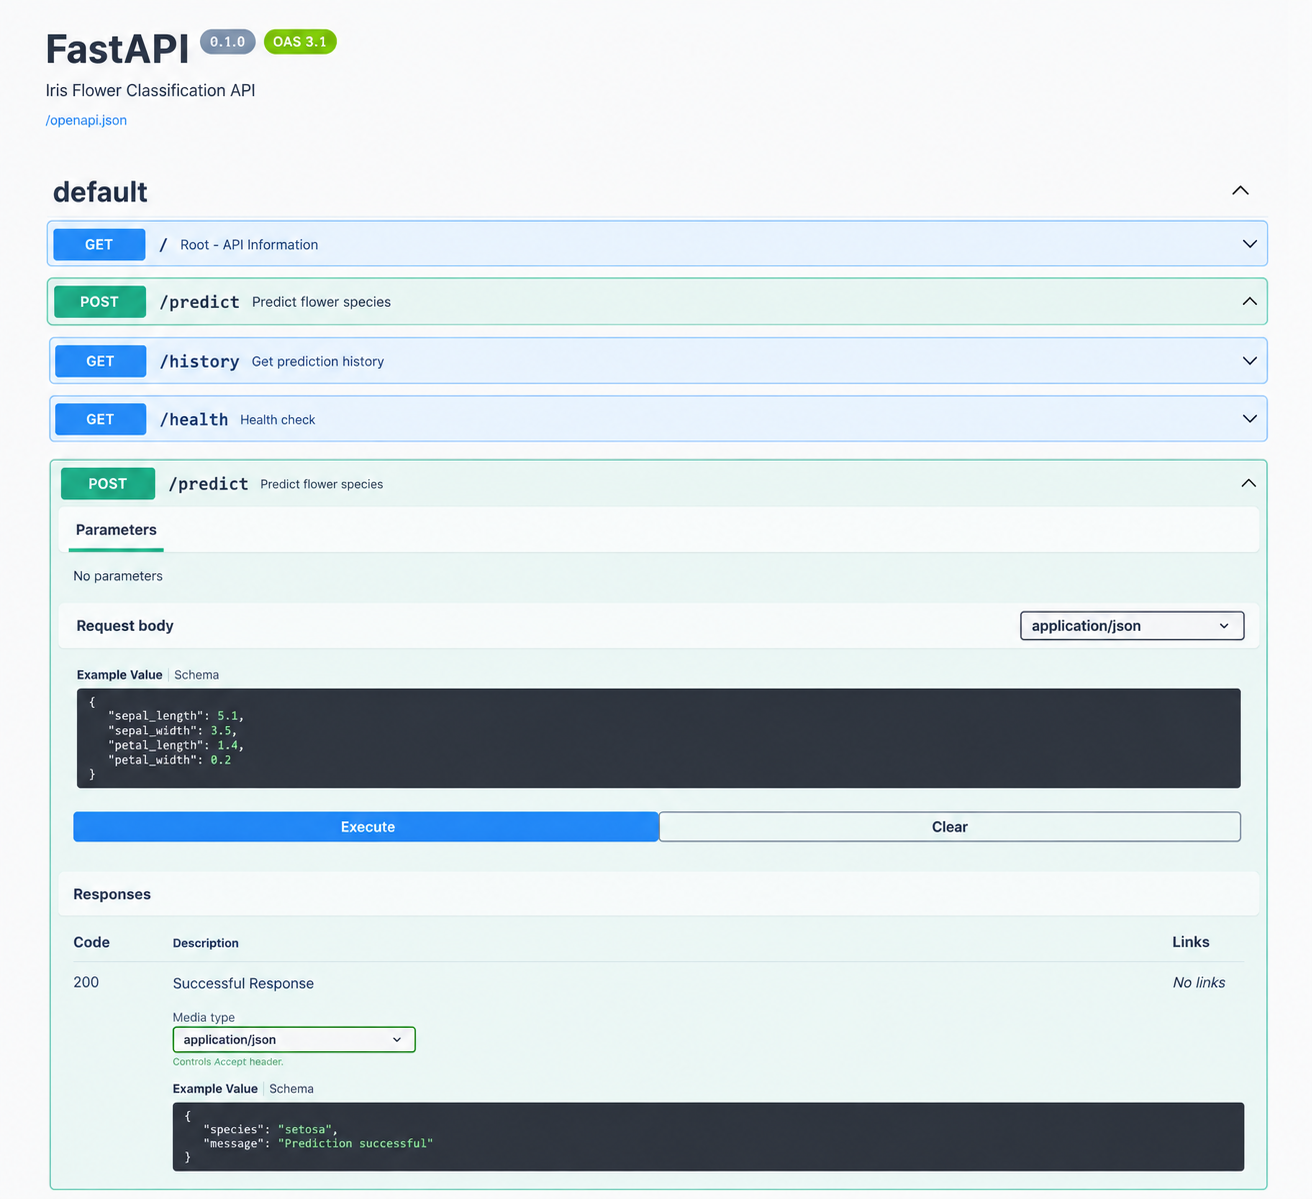
\includegraphics[width=0.6\textwidth]{images/api_predict.png}
		\caption{Kiểm thử API dự đoán thông qua Swagger UI}
		\label{fig:apipredict}
	\end{figure}
	
	\noindent Trong quá trình kiểm thử, dữ liệu đầu vào được truyền dưới dạng JSON. Backend thực hiện kiểm tra dữ liệu, gọi mô hình SVM và trả về kết quả phân loại.
	
	\noindent Một phản hồi thành công có thể có dạng:
	\begin{lstlisting}[language={}, numbers=none, frame=single, basicstyle=\ttfamily\small]
		{6
			"input": {
				"sepal_length": 5.1,
				"sepal_width": 3.5,
				"petal_length": 1.4,
				"petal_width": 0.2
			},
			"prediction_id": 0,
			"predicted_class": "Iris-setosa"
		}
	\end{lstlisting}
	
	
	\noindent Kết quả trên cho thấy API đã tiếp nhận đúng bốn đặc trưng đầu vào và trả về nhãn dự đoán tương ứng. Qua đó kiểm chứng được sự kết nối giữa Frontend, FastAPI Backend và mô hình SVM.
	
	\subsection{Kiểm thử chức năng người dùng}
	
	\noindent Hệ thống người dùng được kiểm tra thông qua các thao tác đăng ký, đăng nhập và duy trì phiên đăng nhập.
	
	\subsubsection{Kiểm thử đăng ký tài khoản}
	
	\noindent Người dùng nhập tên đăng nhập và mật khẩu vào biểu mẫu đăng ký. Hệ thống kiểm tra tính hợp lệ của dữ liệu trước khi tạo tài khoản mới.
	
	\noindent Trường hợp tên đăng nhập chưa tồn tại, thông tin người dùng được ghi vào cơ sở dữ liệu. Nếu tên đăng nhập đã tồn tại, hệ thống trả về thông báo phù hợp và không tạo bản ghi trùng lặp.
	
	\subsubsection{Kiểm thử đăng nhập}
	
	\noindent Khi người dùng nhập thông tin đăng nhập, Backend thực hiện đối chiếu dữ liệu với thông tin đã lưu trong cơ sở dữ liệu.
	
	\noindent Nếu thông tin chính xác, hệ thống tạo phiên đăng nhập và cho phép người dùng tiếp tục sử dụng các chức năng được bảo vệ. Nếu thông tin không chính xác, hệ thống trả về thông báo lỗi tương ứng.
	
	\subsubsection{Kiểm thử quản lý phiên}
	
	\noindent Sau khi đăng nhập thành công, hệ thống duy trì thông tin phiên để xác định tài khoản đang sử dụng. Khi người dùng đăng xuất, phiên hiện tại được kết thúc nhằm ngăn việc tiếp tục sử dụng trạng thái đăng nhập cũ.
	
	\subsection{Kiểm thử lưu trữ dữ liệu}
	
	\noindent Một trong những chức năng được bổ sung trong quá trình hoàn thiện sản phẩm là khả năng lưu trữ dữ liệu hoạt động của người dùng vào cơ sở dữ liệu.
	
	\noindent Các thông tin có thể được ghi nhận bao gồm tài khoản người dùng, thời gian đăng nhập, dữ liệu đầu vào của quá trình dự đoán, kết quả dự đoán và thông tin về thời gian xử lý mô hình.
	
	\subsection{Kiểm thử lịch sử dự đoán}
	
	\noindent Sau khi thực hiện dự đoán, thông tin về kết quả được ghi nhận vào lịch sử tương ứng với tài khoản đang đăng nhập. Người dùng có thể xem lại các lần dự đoán trước đó thông qua chức năng lịch sử trên giao diện.
	
	\noindent Việc xây dựng lịch sử dự đoán giúp phân biệt giữa quá trình xử lý hiện tại và dữ liệu đã phát sinh trước đó, đồng thời tạo nền tảng cho các chức năng quản lý dữ liệu như xóa mềm, khôi phục hoặc xóa vĩnh viễn.
	
	\subsection{Kiểm thử thời gian chạy mô hình}
	
	\noindent Để đánh giá khả năng đáp ứng của hệ thống Web, thời gian xử lý mô hình được ghi nhận trong quá trình thực hiện dự đoán.
	
	\noindent Thời gian này được xác định trong khoảng thời gian hệ thống thực hiện quá trình suy luận với mô hình SVM. Giá trị được ghi nhận giúp theo dõi hiệu năng thực tế của mô hình khi được tích hợp vào Backend.
	
	\noindent Việc ghi nhận thời gian chạy không thay thế cho các chỉ số đánh giá độ chính xác của mô hình. Hai nhóm chỉ số có mục đích khác nhau: các chỉ số như Accuracy, Precision, Recall và F1-score đánh giá chất lượng phân loại, trong khi thời gian chạy phản ánh hiệu năng xử lý của hệ thống.
	
	\subsection{Đánh giá kết quả vận hành}
	
	\noindent Qua các thử nghiệm, hệ thống đã hoàn thành chuỗi xử lý từ tiếp nhận dữ liệu người dùng, kiểm tra dữ liệu, gọi mô hình SVM, trả kết quả dự đoán và lưu trữ thông tin vào cơ sở dữ liệu.
	
	\noindent Quá trình kiểm thử cho thấy các thành phần của hệ thống có thể phối hợp theo đúng luồng thiết kế:
	
	\begin{center}
		\textbf{Người dùng}
		$\rightarrow$
		\textbf{Web}
		$\rightarrow$
		\textbf{FastAPI}
		$\rightarrow$
		\textbf{SVM}
		$\rightarrow$
		\textbf{Kết quả}
		$\rightarrow$
		\textbf{Cơ sở dữ liệu}
	\end{center}
	
	\noindent Như vậy, sản phẩm không chỉ dừng lại ở việc xây dựng và đánh giá một mô hình học máy mà đã được mở rộng thành một hệ thống có khả năng tương tác với người dùng, cung cấp API, quản lý tài khoản và lưu trữ dữ liệu phục vụ quá trình vận hành.
	

	\newpage 

	
	
	% ============================================================
	% PHỤ LỤC
	% ============================================================
	
	\newpage
	\section*{PHỤ LỤC}
	\addcontentsline{toc}{section}{PHỤ LỤC}
	
	\noindent
	Phần phụ lục trình bày các thành phần quan trọng được sử dụng trong quá
	trình xây dựng và vận hành hệ thống \textbf{IRIS BOTANICA AI}. Nội dung
	được tổ chức theo từng nhóm nhằm giúp người đọc dễ dàng theo dõi quá trình
	từ huấn luyện mô hình, xây dựng API, kết nối cơ sở dữ liệu đến vận hành
	ứng dụng Web.
	
	\noindent
	Toàn bộ mã nguồn của đề tài được nộp riêng kèm theo sản phẩm. Vì vậy,
	phần phụ lục chỉ trình bày các đoạn mã tiêu biểu và hướng dẫn cần thiết
	để kiểm tra, sử dụng và vận hành hệ thống.
	
	
	% ============================================================
	% PHỤ LỤC A
	% ============================================================
	
	
	\subsection*{Phụ lục A. Hướng dẫn khởi chạy hệ thống}
	\addcontentsline{toc}{subsection}{Phụ lục A. Hướng dẫn khởi chạy hệ thống}
	
	\noindent
	Phần này trình bày các bước cần thực hiện để khởi động hệ thống
	\textbf{IRIS BOTANICA AI} trên môi trường máy tính cục bộ.
	
	\subsubsection*{A.1. Chuẩn bị môi trưường}
	
	\noindent
	Trước khi khởi chạy hệ thống, cần chuẩn bị:
	
	\begin{itemize}[leftmargin=*]
		\item Python 3.12 hoặc phiên bản tương thích.
		\item Visual Studio Code hoặc môi trường lập trình Python tương đương.
		\item Các thư viện được khai báo trong tệp \text{requirements.txt}.
		\item Toàn bộ mã nguồn của dự án \text{SVM-IRIS}.
		\item Tệp mô hình đã huấn luyện \text{svm\_model.pkl}.
		\item Cơ sở dữ liệu \texttt{iris\_database.db}.
	\end{itemize}
	
	\subsubsection*{A.2. Mở thư mục dự án}
	
	\noindent
	Mở thư mục chứa dự án \texttt{SVM-IRIS} bằng Visual Studio Code.
	Kiểm tra để đảm bảo các tệp chính của hệ thống đã được đặt đúng vị trí.
	\begin{folderbox}[Cấu trúc thư mục dự án IRIS BOTANICA AI]
		
		\begin{forest}
			for tree={
				font=\small\ttfamily,
				grow'=0,
				child anchor=west,
				parent anchor=south west,
				anchor=west,
				l sep=5pt,
				s sep=2pt,
				edge path={
					\noexpand\path[draw]
					(!u.parent anchor) ++(3pt,0) |- (.child anchor);
				}
			}
			[IRIS-BOTANICA-AI
			[app.py]
			[TRAIN\_SVM.py]
			[evaluate\_models.py]
			[index.html]
			[database
			[connection.py]
			[user.py]
			[history.py]
			[prediction.py]
			[model.py]
			[model\_history.py]
			]
			[SQL]
			[images]
			[report]
			[Iris.csv]
			[svm\_model.pkl]
			[lda\_model.pkl]
			[knn\_model.pkl]
			[requirements.txt]
			[Procfile]
			[render.yaml]
			]
		\end{forest}
		
	\end{folderbox}
	
	\subsubsection*{A.3. Khởi động máy chủ FastAPI}
	
	\noindent
	Mở Terminal tại thư mục dự án và thực hiện lệnh:
	
	\begin{lstlisting}[language=bash,
		numbers=none,
		frame=single,
		basicstyle=\ttfamily\small]
		python -m uvicorn app:app --reload
	\end{lstlisting}
	
	\noindent
	Tham số \text{--reload} cho phép máy chủ tự động khởi động lại khi
	mã nguồn được thay đổi trong quá trình phát triển.
	
	\noindent
	Nếu khởi động thành công, Terminal sẽ hiển thị thông báo máy chủ đang
	chạy tại địa chỉ cục bộ.
	
	newpage
	\newpage
	\subsubsection*{A.4. Kiểm tra hệ thống}
	
	\noindent
	Sau khi máy chủ được khởi động, mở trình duyệt và truy cập:
	
	\begin{center}
		\texttt{http://127.0.0.1:8000}
	\end{center}
	
	\noindent
	Để kiểm tra các API thông qua giao diện Swagger UI, truy cập:
	
	\begin{center}
		\texttt{http://127.0.0.1:8000/docs}
	\end{center}
	
	
	
	
	% ============================================================
	% PHỤ LỤC B
	% ============================================================
	
	
	\subsection*{Phụ lục B. Hướng dẫn sử dụng Web IRIS BOTANICA AI}
	\addcontentsline{toc}{subsection}{Phụ lục B. Hướng dẫn sử dụng Web IRIS BOTANICA AI}
	
	\noindent
	Phần này trình bày quy trình sử dụng sản phẩm từ khi người dùng truy cập
	hệ thống đến khi nhận được kết quả phân loại hoa Iris.
	
	\subsubsection*{B.1. Truy cập hệ thống}
	
	\noindent
	Người dùng truy cập địa chỉ Web của hệ thống
	\textbf{IRIS BOTANICA AI} bằng trình duyệt.
	
	\subsubsection*{B.2. Đăng ký tài khoản}
	
	\noindent
	Người dùng lựa chọn chức năng đăng ký và nhập thông tin tài khoản theo
	yêu cầu của hệ thống.
	
	\noindent
	Sau khi đăng ký thành công, thông tin người dùng được lưu vào cơ sở
	dữ liệu để phục vụ quá trình đăng nhập và quản lý lịch sử sử dụng.
	
	
	\subsubsection*{B.3. Đăng nhập}
	
	\noindent
	Người dùng nhập tên đăng nhập và mật khẩu đã đăng ký. Hệ thống kiểm tra
	thông tin với dữ liệu được lưu trong cơ sở dữ liệu.
	
	\noindent
	Nếu thông tin hợp lệ, người dùng được xác thực và có thể sử dụng các
	chức năng của hệ thống.
	
	\subsubsection*{B.4. Nhập thông số hoa Iris}
	
	\noindent
	Người dùng nhập bốn thông số hình thái của mẫu hoa:
	
	\begin{itemize}[leftmargin=*]
		\item Chiều dài đài hoa.
		\item Chiều rộng đài hoa.
		\item Chiều dài cánh hoa.
		\item Chiều rộng cánh hoa.
	\end{itemize}
	
	\noindent
	Các thông số này được sử dụng làm dữ liệu đầu vào cho mô hình SVM.
	
	
	\subsubsection*{B.5. Thực hiện dự đoán}
	
	\noindent
	Sau khi nhập đầy đủ dữ liệu, người dùng nhấn nút dự đoán. Giao diện Web
	gửi yêu cầu đến API \texttt{/predict}.
	
	\noindent
	API tiếp nhận dữ liệu, đưa dữ liệu vào mô hình SVM và trả về kết quả
	phân loại.
	
	\subsubsection*{B.6. Hiển thị kết quả}
	
	\noindent
	Kết quả dự đoán được hiển thị trực tiếp trên giao diện Web. Hệ thống
	có thể trả về một trong ba lớp:
	
	\begin{itemize}[leftmargin=*]
		\item \textit{Iris-setosa}.
		\item \textit{Iris-versicolor}.
		\item \textit{Iris-virginica}.
	\end{itemize}
	
	
	
	\subsubsection*{B.7. Xem lịch sử sử dụng}
	
	\noindent
	Sau khi thực hiện dự đoán, kết quả được lưu trữ để người dùng có thể
	xem lại lịch sử sử dụng của mình.
	
	
	
	% ============================================================
	% PHỤ LỤC C
	% ============================================================
	
	
	\subsection*{Phụ lục C. Hướng dẫn kiểm thử API}
	\addcontentsline{toc}{subsection}{Phụ lục C. Hướng dẫn kiểm thử API}
	
	\noindent
	Hệ thống cung cấp giao diện Swagger UI giúp kiểm tra trực tiếp các
	API mà không cần sử dụng thêm công cụ bên ngoài.
	
	\subsubsection*{C.1. Mở giao diện kiểm thử API}
	
	\noindent
	Truy cập:
	
	\begin{center}
		\texttt{http://127.0.0.1:8000/docs}
	\end{center}
	
	
	\subsubsection*{C.2. Kiểm thử API dự đoán}
	
	\noindent
	Chọn API:
	
	\begin{center}
		\texttt{POST /predict}
	\end{center}
	
	\noindent
	Sau đó chọn chức năng \text{Try it out} và nhập dữ liệu kiểm thử.
	
	\begin{lstlisting}[numbers=none,
		frame=single,
		basicstyle=\ttfamily\small]
		{
			"sepal_length": 5.1,
			"sepal_width": 3.5,
			"petal_length": 1.4,
			"petal_width": 0.2
		}
	\end{lstlisting}
	
	\noindent
	Sau khi nhấn \text{Execute}, hệ thống trả về kết quả dưới dạng JSON.
	
	\begin{lstlisting}[numbers=none,
		frame=single,
		basicstyle=\ttfamily\small]
		{
			"prediction_id": 0,
			"predicted_class": "Iris-setosa"
		}
	\end{lstlisting}
	
	
	\subsubsection*{C.3. Kiểm tra dữ liệu không hợp lệ}
	
	\noindent
	Có thể nhập dữ liệu không đúng kiểu hoặc bỏ trống trường dữ liệu để
	kiểm tra khả năng xác thực dữ liệu của API.
	
	\noindent
	FastAPI và Pydantic sẽ phát hiện dữ liệu không hợp lệ và trả về thông
	báo lỗi tương ứng.
	
	
	% ============================================================
	% PHỤ LỤC D
	% ============================================================
	
	\newpage
	\subsection*{Phụ lục D. Hướng dẫn kiểm tra cơ sở dữ liệu}
	\addcontentsline{toc}{subsection}{Phụ lục D. Hướng dẫn kiểm tra cơ sở dữ liệu}
	
	\noindent
	Cơ sở dữ liệu được sử dụng để lưu trữ các thông tin phát sinh trong quá
	trình sử dụng hệ thống.
	
	\subsubsection*{D.1. Kiểm tra thông tin người dùng}
	
	\noindent
	Sau khi đăng ký tài khoản, thông tin người dùng được lưu vào bảng
	tương ứng trong cơ sở dữ liệu.
	
	
	\subsubsection*{D.2. Kiểm tra lịch sử đăng nhập}
	
	\noindent
	Mỗi lần người dùng đăng nhập thành công, hệ thống ghi nhận thông tin
	lịch sử đăng nhập nhằm phục vụ quản lý và kiểm tra hoạt động của hệ thống.
	
	
	
	\subsubsection*{D.3. Kiểm tra lịch sử dự đoán}
	
	\noindent
	Khi người dùng thực hiện dự đoán, dữ liệu đầu vào và kết quả phân loại
	được lưu vào cơ sở dữ liệu.
	
	\noindent
	Thông tin này cho phép người dùng xem lại các lần dự đoán trước đó và
	giúp hệ thống quản lý lịch sử sử dụng.
	
	\subsubsection*{D.4. Đối chiếu dữ liệu giữa Web và cơ sở dữ liệu}
	
	\noindent
	Quá trình lưu trữ dữ liệu được kiểm tra bằng cách thực hiện một thao tác
	trên Web, sau đó kiểm tra lại bản ghi tương ứng trong cơ sở dữ liệu.
	
	\begin{center}
		\textbf{
			Người dùng
			$\rightarrow$
			Web
			$\rightarrow$
			API
			$\rightarrow$
			Cơ sở dữ liệu
		}
	\end{center}
	
	\noindent
	Cách kiểm tra này giúp xác nhận dữ liệu được truyền và lưu trữ đúng
	giữa các thành phần của hệ thống.
	
	
	% ============================================================
	% PHỤ LỤC E
	% ============================================================
	
	
	\subsection*{Phụ lục E. Cấu trúc thư mục sản phẩm}
	\addcontentsline{toc}{subsection}{Phụ lục E. Cấu trúc thư mục sản phẩm}
	
	\noindent
	Dự án được tổ chức thành các thành phần tương ứng với từng chức năng
	của hệ thống:
	\newpage 
	\begin{lstlisting}[language={},
		numbers=none,
		frame=single,
		basicstyle=\ttfamily\small]
		SVM-IRIS/
		│
		├── app.py
		├── TRAIN_SVM.py
		├── svm_model.pkl
		├── Iris.csv
		├── requirements.txt
		├── Procfile
		├── render.yaml
		├── index.html
		│
		├── images/
		│
		├── database/
		│   ├── connection.py
		│   ├── model.py
		│   └── ...
		│
		├── charts/
		│   └── confusion_matrix.py
		│
		└── iris_database.db
	\end{lstlisting}
	
	\noindent
	Trong đó:
	
	\begin{itemize}[leftmargin=*]
		\item \texttt{TRAIN\_SVM.py}: chương trình huấn luyện và đánh giá
		mô hình SVM.
		
		\item \texttt{svm\_model.pkl}: tệp lưu mô hình SVM đã huấn luyện.
		
		\item \texttt{app.py}: chương trình Backend và các API của hệ thống.
		
		\item \texttt{index.html}: giao diện Web của sản phẩm.
		
		\item \texttt{database/}: các thành phần kết nối và thao tác với
		cơ sở dữ liệu.
		
		\item \texttt{charts/}: các chương trình tạo biểu đồ đánh giá và
		trực quan hóa dữ liệu.
		
		\item \texttt{iris\_database.db}: cơ sở dữ liệu của hệ thống.
	\end{itemize}
	
	
	% ============================================================
	% PHỤ LỤC F
	% ============================================================
	
	
	\subsection*{Phụ lục F. Quy trình vận hành sản phẩm}
	\addcontentsline{toc}{subsection}{Phụ lục F. Quy trình vận hành sản phẩm}
	
	\noindent
	Toàn bộ hệ thống được vận hành theo quy trình từ mô hình học máy đến
	ứng dụng Web như sau:
	
	\begin{center}
		\textbf{
			Dữ liệu Iris
			$\rightarrow$
			Huấn luyện SVM
			$\rightarrow$
			Đánh giá mô hình
			$\rightarrow$
			Lưu mô hình
		}
	\end{center}
	
	\begin{center}
		\textbf{
			$\downarrow$
		}
	\end{center}
	
	\begin{center}
		\textbf{
			FastAPI
			$\rightarrow$
			API dự đoán
			$\rightarrow$
			Cơ sở dữ liệu
			$\rightarrow$
			Giao diện Web
		}
	\end{center}
	
	\begin{center}
		\textbf{
			$\downarrow$
		}
	\end{center}
	
	\begin{center}
		\textbf{
			Người dùng
			$\rightarrow$
			Nhập dữ liệu
			$\rightarrow$
			Dự đoán
			$\rightarrow$
			Lưu lịch sử
		}
	\end{center}
	
	\subsubsection*{F.1. Các bước vận hành}
	
	\begin{enumerate}[leftmargin=*]
		
		\item Chuẩn bị tập dữ liệu Iris và mã nguồn của dự án.
		
		\item Huấn luyện mô hình SVM với Kernel tuyến tính.
		
		\item Đánh giá hiệu quả của mô hình trên tập kiểm thử.
		
		\item Huấn luyện mô hình cuối cùng và lưu thành
		\texttt{svm\_model.pkl}.
		
		\item Khởi động máy chủ FastAPI.
		
		\item Kiểm tra API thông qua Swagger UI.
		
		\item Kết nối hệ thống với cơ sở dữ liệu.
		
		\item Truy cập giao diện Web IRIS BOTANICA AI.
		
		\item Đăng ký hoặc đăng nhập tài khoản.
		
		\item Nhập bốn thông số của mẫu hoa Iris.
		
		\item Gửi yêu cầu dự đoán.
		
		\item API gọi mô hình SVM và trả về kết quả.
		
		\item Hệ thống lưu thông tin cần thiết vào cơ sở dữ liệu.
		
		\item Người dùng có thể xem lại lịch sử sử dụng.
		
	\end{enumerate}
	
	\subsubsection*{F.2. Kết quả vận hành}
	
	\noindent
	Sau khi hoàn thành các bước trên, hệ thống có khả năng thực hiện đầy đủ
	chu trình từ dữ liệu đầu vào đến kết quả dự đoán trên giao diện Web.
	
	
	\noindent
	Địa chỉ sản phẩm trực tuyến:
	
	\begin{center}
		\url{https://iris-svm-api-4c5t.onrender.com/}
	\end{center}
	
	
	
	\noindent
	\textbf{Ghi chú:} Toàn bộ mã nguồn đầy đủ của sản phẩm được cung cấp
	riêng kèm theo báo cáo. Phần phụ lục có mục đích minh họa các thành phần
	quan trọng và cung cấp hướng dẫn kiểm tra, sử dụng và vận hành hệ thống.
	
	
	% Đổi tên tiêu đề mặc định của môi trường bibliography thành tiếng Việt
	\renewcommand{\refname}{TÀI LIỆU THAM KHẢO}
	\addcontentsline{toc}{section}{TÀI LIỆU THAM KHẢO}
	
	\begin{thebibliography}{99}
		
		\bibitem{scikit-learn}
		Học máy cơ bản, Tôn Thất Tú(2025) 
		
		\bibitem{iris-dataset}
		Fisher, R. A. (1936). 
		\textit{The use of multiple measurements in taxonomic problems}. 
		Annals of Eugenics, 7(2), 179-188.
		
		\bibitem{fastapi}2025
		Tiangolo (Sebastián Ramírez). (2018). 
		\textit{FastAPI framework, high performance, easy to learn, fast to code, ready for production}. 
		Trang chủ: \url{https://fastapi.tiangolo.com/}.
		
		\bibitem{github-pages}
		GitHub Documentation. (2024). 
		\textit{GitHub Pages Overview}. 
		Truy cập tại: \url{https://docs.github.com/en/pages}.
		
		\bibitem{render-docs}
		Render Cloud Documentation. (2024). 
		\textit{Deploying Python Web Services on Render}. 
		Truy cập tại: \url{https://render.com/docs}.
		
	\end{thebibliography}
	
\end{document}